\documentclass[10pt, landscape]{article}
\usepackage[scaled=0.92]{helvet}
\usepackage{calc}
\usepackage{multicol}
\usepackage[a4paper,margin=3mm,landscape]{geometry}
\usepackage{amsmath,amsthm,amsfonts,amssymb}
\usepackage{color,graphicx,overpic}
\usepackage{hyperref}
\usepackage{newtxtext} 
\usepackage{enumitem}
\usepackage[table]{xcolor}
\usepackage{mathtools}
\setlist{nosep}
\usepackage{tikz}
\usetikzlibrary{shapes.geometric}
\usepackage{makecell}  % for line break withih tabular

% for including images
\graphicspath{ {../images/} }


\pdfinfo{
  /Title (CS2102.pdf)
  /Creator (TeX)
  /Producer (pdfTeX 1.40.0)
  /Author (Jovyn Tan)
  /Subject (CS2102)
/Keywords (CS2102, nus,cheatsheet,pdf)}

% Turn off header and footer
\pagestyle{empty}

% redefine section commands to use less space
\makeatletter
\renewcommand{\section}{\@startsection{section}{1}{0mm}%
  {-1ex plus -.5ex minus -.2ex}%
  {0.5ex plus .2ex}%x
{\normalfont\large\bfseries}}
\renewcommand{\subsection}{\@startsection{subsection}{2}{0mm}%
  {-1explus -.5ex minus -.2ex}%
  {0.5ex plus .2ex}%
{\normalfont\normalsize\bfseries}}
\renewcommand{\subsubsection}{\@startsection{subsubsection}{3}{0mm}%
  {-1ex plus -.5ex minus -.2ex}%
  {1ex plus .2ex}%
{\normalfont\small\bfseries}}%
\makeatother

\renewcommand{\familydefault}{\sfdefault}
\renewcommand\rmdefault{\sfdefault}
%  makes nested numbering (e.g. 1.1.1, 1.1.2, etc)
\renewcommand{\labelenumii}{\theenumii}
\renewcommand{\theenumii}{\theenumi.\arabic{enumii}.}
\renewcommand\labelitemii{•}
\renewcommand\labelitemiii{•}

\definecolor{mathblue}{cmyk}{1,.72,0,.38}
\everymath\expandafter{\the\everymath \color{mathblue}}

% Don't print section numbers
\setcounter{secnumdepth}{0}

\setlength{\parindent}{0pt}
\setlength{\parskip}{0pt plus 0.5ex}
%% this changes all items (enumerate and itemize)
\setlength{\leftmargini}{0.5cm}
\setlength{\leftmarginii}{0.5cm}
\setlist[itemize,1]{leftmargin=2mm,labelindent=1mm,labelsep=1mm}
\setlist[itemize,2]{leftmargin=2mm,labelindent=1mm,labelsep=1mm}
\setlist[itemize,3]{leftmargin=2mm,labelindent=1mm,labelsep=1mm}

% adding my commands
% tightcenter
\newenvironment{tightcenter}{%
  \setlength\topsep{0pt}
  \setlength\parskip{0pt}
  \begin{center}
    }{%
  \end{center}
}

% boxed
\newenvironment{tightbox}{%
  \setlength\topsep{0pt}
  \setlength\parskip{0pt}
  \begin{center}
    \begin{tabular}{|@{\hspace{\dimexpr\fboxsep+0.5\arrayrulewidth}}c@{\hspace{\dimexpr\fboxsep+0.5\arrayrulewidth}}|}
      \hline
    }
    {%
    \\ \hline
    \end{tabular}
  \end{center}
}

% fixed width box
\newenvironment{fixedbox}[1][0.7]{
  \setlength\topsep{0pt}
  \setlength\parskip{0pt}
  \begin{center}
    \begin{tabular}{|>{\centering\arraybackslash}m{#1\linewidth}|}
    \hline
  }{
  \\ \hline
  \end{tabular}
  \end{center}
}

% definition of a new term
\usepackage{soul}
\definecolor{paleyellow}{RGB}{251,243,218}
\newcommand{\definition}[2][]{\sethlcolor{paleyellow}\hl{\textbf{#2}} #1  $\rightarrow$}
% inline definition
\newcommand{\ildefinition}[1]{\sethlcolor{paleyellow}\hl{\textbf{#1}}}

% important note (attention)
\newcommand{\attention}{{\color{red}\textbf{! }}}

% nice proof
\newenvironment{niceproof}[1][Proof]
{%
  \sbox0{\textit{#1}. }%
  \list{}{\labelwidth\wd0 \leftmargin\wd0 \labelsep 0pt }
\item[\usebox0]}
  {\endlist}


\usepackage{color, soul}
\usepackage{listings}
\usepackage{inconsolata}

\definecolor{codegreen}{rgb}{0,0.6,0}
\definecolor{codegray}{rgb}{0.5,0.5,0.5}
\definecolor{codepurple}{HTML}{C42043}
\definecolor{backcolour}{HTML}{F2F2F2}
\definecolor{bookColor}{cmyk}{0,0,0,0.90}

\newcommand{\code}[1]{\texttt{\sethlcolor{backcolour}\hl{$\,$#1$\,$}}}

% SQL code blocks
% define SQL styles
\lstdefinestyle{mySQL}{%
  language=SQL,
  backgroundcolor=\color{backcolour},
  commentstyle=\color{codegreen},
  keywordstyle=\color{codepurple},
  numberstyle=\numberstyle,
  stringstyle=\color{codepurple},
  basicstyle=\scriptsize\ttfamily,
  breaklines=true,
}

%  convenient absolute value symbol
\newcommand{\abs}[1]{\vert #1 \vert}

%  convenient floor and ceiling
\newcommand{\floor}[1]{\lfloor #1 \rfloor}
\newcommand{\ceil}[1]{\lceil #1 \rceil}

%  modulo with nicer spacing
\newcommand{\Mod}[1]{\ \mathrm{mod}\ #1}

%  convenient dx with nicer spacing
\newcommand{\dx}{\mathop{dx}}
\newcommand{\dy}{\mathop{dy}}


\usepackage{amssymb}

\DeclareRobustCommand{\ojoin}{\setbox0=\hbox{$\bowtie$}%
  \rule[-.02ex]{.25em}{.4pt}\llap{\rule[\ht0]{.25em}{.4pt}}}
\def\leftouterjoin{\mathbin{\ojoin\mkern-5.8mu\bowtie}}
\def\rightouterjoin{\mathbin{\bowtie\mkern-5.8mu\ojoin}}
\def\fullouterjoin{\mathbin{\ojoin\mkern-5.8mu\bowtie\mkern-5.8mu\ojoin}}

\newcommand\lojoin{\leftouterjoin}
\newcommand\rojoin{\rightouterjoin}
\newcommand\fojoin{\fullouterjoin}

% -----------------------------------------------------------------------

\begin{document}
\raggedright
\footnotesize
\begin{multicols}{4}

  % multicol parameters
  % These lengths are set only within the two main columns
  \setlength{\columnseprule}{0.25pt}
  \setlength{\premulticols}{1pt}
  \setlength{\postmulticols}{1pt}
  \setlength{\multicolsep}{1pt}
  \setlength{\columnsep}{2pt}

  \begin{center}
    \fbox{%
      \parbox{0.8\linewidth}{\centering \textcolor{black}{
          {\Large\textbf{CS2102}}
        \\ \normalsize{AY21/22 SEM 1}}
        \\ {\footnotesize \textcolor{gray}{github/jovyntls}}
      }%
    }
  \end{center}

  \section{DBMS}
  \subsection{Transactions}
  \begin{itemize}
    \item \definition{transaction, $T$} a finite sequence of database operations
    \item 4 properties of a transaction: \textbf{ACID} properties
  \end{itemize}

  \textbf{ACID properties}
  \begin{enumerate}
    \item \textbf{Atomicity} \(\rightarrow\) either all effects of $ T $ are reflected in the database, or none
    \item \textbf{Consistency}  \(\rightarrow\) the execution of $ T $ guarantees to yield a \textit{correct state} of the DB
    \item \textbf{Isolation} \(\rightarrow\)  execution of T is \textit{isolated} from the effects of concurrent transactions
    \item \textbf{Durability} \(\rightarrow\) after the commit of $ T $, its effects are \textit{permanent}  in case of failures
  \end{enumerate}

  \subsubsection{Serializability}
  \begin{itemize}
    \item Requirement for Concurrent Execution: \textbf{serializable transaction execution} 
      \begin{itemize}
        \item concurrency: to optimise performance
        \item serializability: to ensure integrity of data
      \end{itemize}
    \item (concurrent execution of a set of transactions is) \definition{serializable} execution is equivalent to some serial execution of the same set of transactions
      \begin{itemize}
        \item \definition{equivalent} they have the same \textit{effect}  on the data
      \end{itemize}
  \end{itemize}

  \section{RELATIONAL MODEL}
  \begin{tightcenter}
    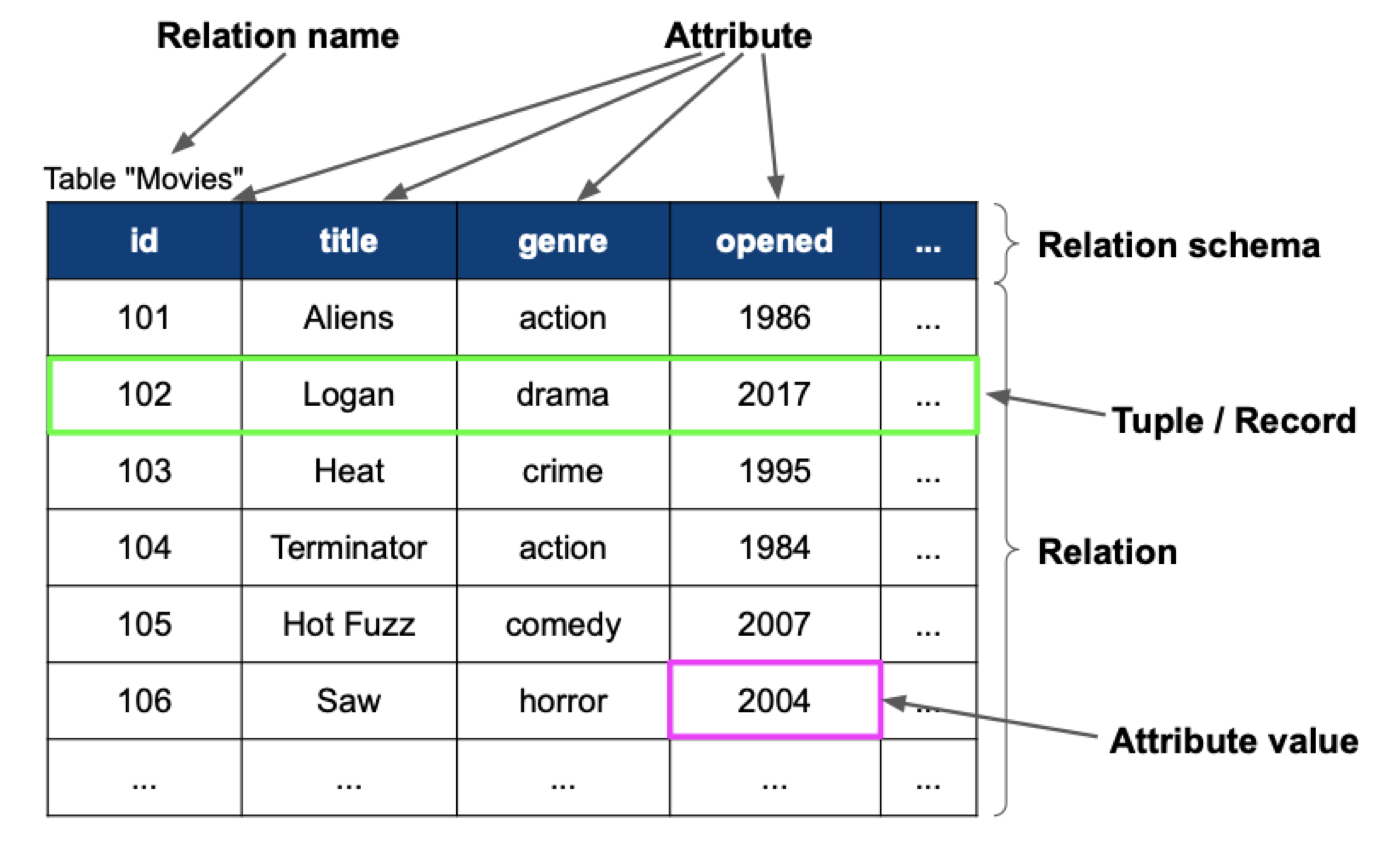
\includegraphics[width=0.7\linewidth]{cs2102-relational-model-example.png}
  \end{tightcenter}

  \begin{itemize}
    \item \definition{relation schema} defines a relation 
      \begin{itemize}
        \item specifies \textbf{attributes} and data constraints
        \item $ R(A_1, A_2, \dots, A_n) $ : relation schema with name $ R $ and $ n $ attributes $ A_1, A_2, \dots, A_n $
      \end{itemize}
    \item \definition{relational database schema} set of relation schemas + data constraints
      \begin{itemize}
        \item TableName(col\_1, col\_2, col\_3) with dom(col\_1) = \{x, y, z\}
      \end{itemize}
    \item \definition{domain} a set of \textit{atomic} values 
      \begin{itemize}
        \item $ dom(A_i) =$ set of possible values for $ A_i $
          \begin{itemize}
            \item e.g. dom(course) = \{cs2102, cs2030, cs2040\}
          \end{itemize}
        \item for all value $ v $ of attribute $ A_i, v \in \{ dom(A_i) \cup \{null\} \} $ 
      \end{itemize}
    \item \definition{relation} a set of \textit{tuples} 
      \begin{itemize}
        \item each instance of schema $ R $ is a relation which is a subset of $ \{(a_1, a_2, \dots, a_n) \mid a_i \in dom(A_i) \cup \{null\}\} $
      \end{itemize}
    \item \definition{integrity constraint} condition that restricts what constitutes valid data
    \item \definition{structural} (integrity constraint) inherent to the data model 
  \end{itemize}

  \subsection{Key Constraints}
  \begin{itemize}
    \item \definition{superkey} subset of attributes that \textit{uniquely} identifies a tuple in a relation
    \item \definition{key} superkey that is also \textbf{minimal} - no proper subset of the key is a superkey
    \item \definition{candidate keys} set of all keys for a relation
    \item \definition{primary key} selected candidate key; cannot be \code{null}
      \begin{itemize}
        \item \definition{prime attributes} attributes of the primary key
      \end{itemize}
  \end{itemize}

  \section{CONSTRAINTS}
  \begin{itemize}
    \item \textbf{Not-Null Constraints} violation: $\exists t \in$ Employees where \code{t.id IS NOT NULL} evaluates to \textbf{false}
    \item \textbf{Unique Constraints} violation: For any 2 tuples $t_i, t_k \in R$, \\*
      $(t_i\cdot A <> t_k\cdot A)$ or  $(t_i\cdot B <> t_k \cdot B)$ evaluates to  \textbf{false}
      \begin{itemize}
        \item \attention \code{null} rows will NOT violate unique key constraints
      \end{itemize}
    \item \textbf{Primary Key Constraints}: prime attributes cannot be null
      \begin{itemize}
        \item (entity integrity constraint)
      \end{itemize}
    \item \textbf{Foreign Key Constraints}: each FK in the referencing relation \textit{must}:
      \begin{itemize}
        \item appear as a \textbf{PK} in the referenced relation, OR 
        \item be a \code{null} value
      \end{itemize}
    \item \texttt{R.sid} $\rightarrow$ \texttt{S.id}: \texttt{R.sid} is a FK referencing PK \texttt{id} in S
  \end{itemize}

  \section{ENTITY RELATIONSHIP MODEL}
  \begin{itemize}
    \item \definition{entity set} collection of entities of the same type
    \item \definition{attribute} specific information describing an entity
      \begin{itemize}
        \item \definition{key attribute} uniquely identifies each entity 
        \item \definition{composite attribute} composed of multiple other attributes 
        \item \definition{multivalued attribute} may comprise more than one value for a given entity 
        \item \definition{derived attribute} derived from other attributes 
      \end{itemize}
  \end{itemize}
  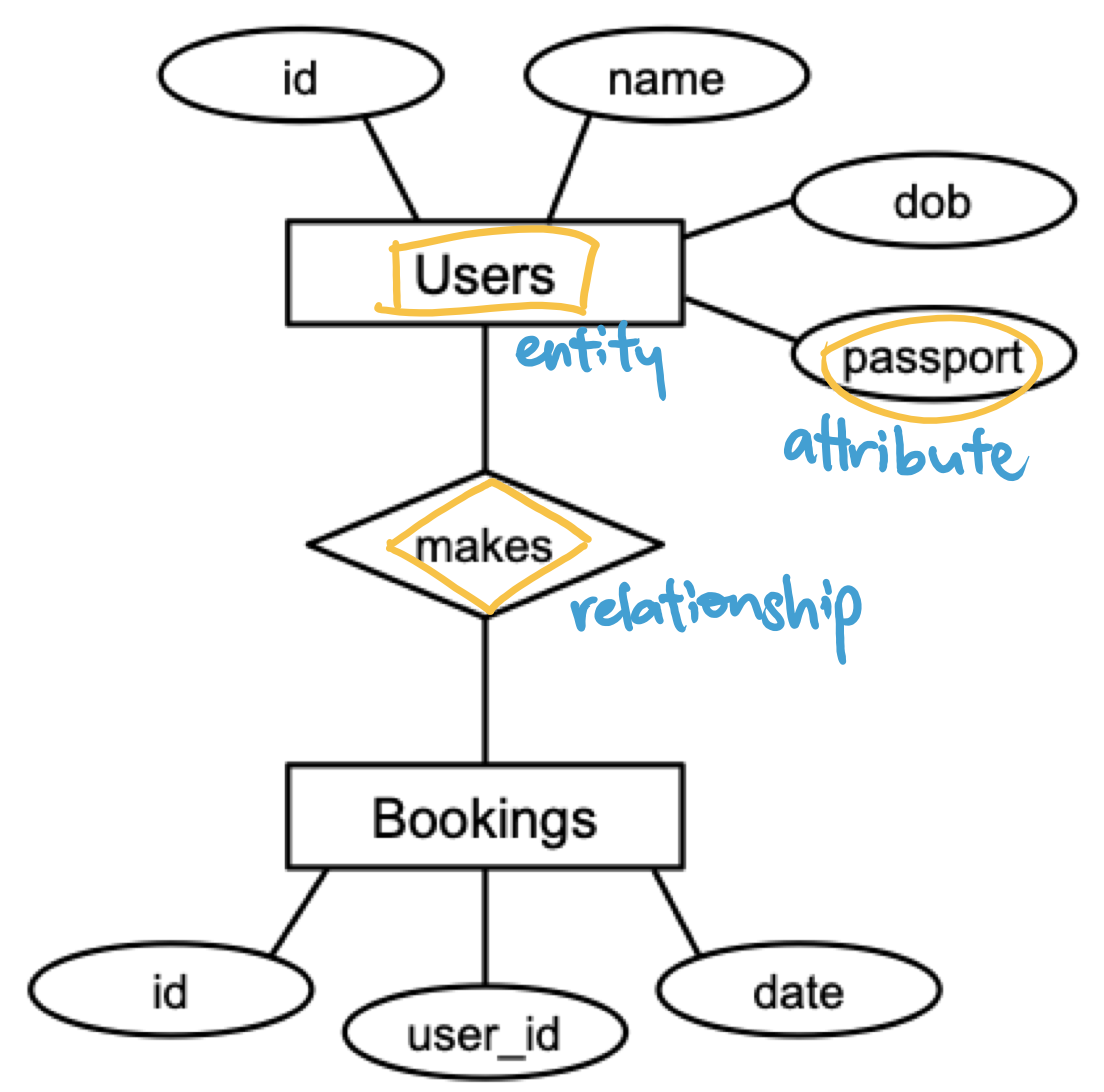
\includegraphics[width=0.4\linewidth]{cs2102-entity-relationship-model.png} 
  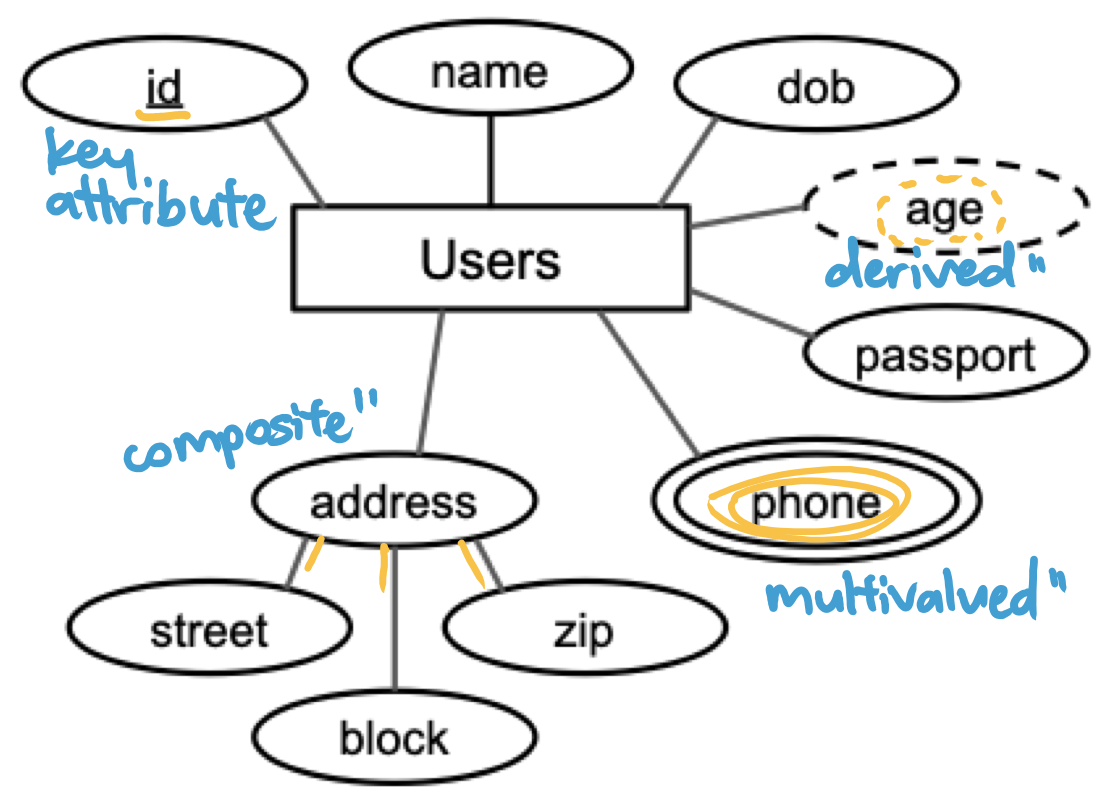
\includegraphics[width=0.55\linewidth]{cs2102-attribute-subtypes.png} 

  \subsubsection{Relationship Sets}
  \begin{itemize}
    \item \definition{degree} no. of entity roles participating in a relationship 
      \begin{itemize}
        \item an $n$-ary relationship set involves $n$ entity roles (where $n$ is the degree of the relationship set)
      \end{itemize}
  \end{itemize}

  \subsection{Dependency Constraints}
  \begin{itemize}
    \item \definition{weak entity sets} entity set that does not have its own key 
      \begin{itemize}
        \item can only be uniquely identified through the primary key of its \textbf{owner entity}
        \item \definition{partial key} set of attributes that uniquely identifies a weak entity for a given owner entity (identifies the exact instance of a weak entity)
          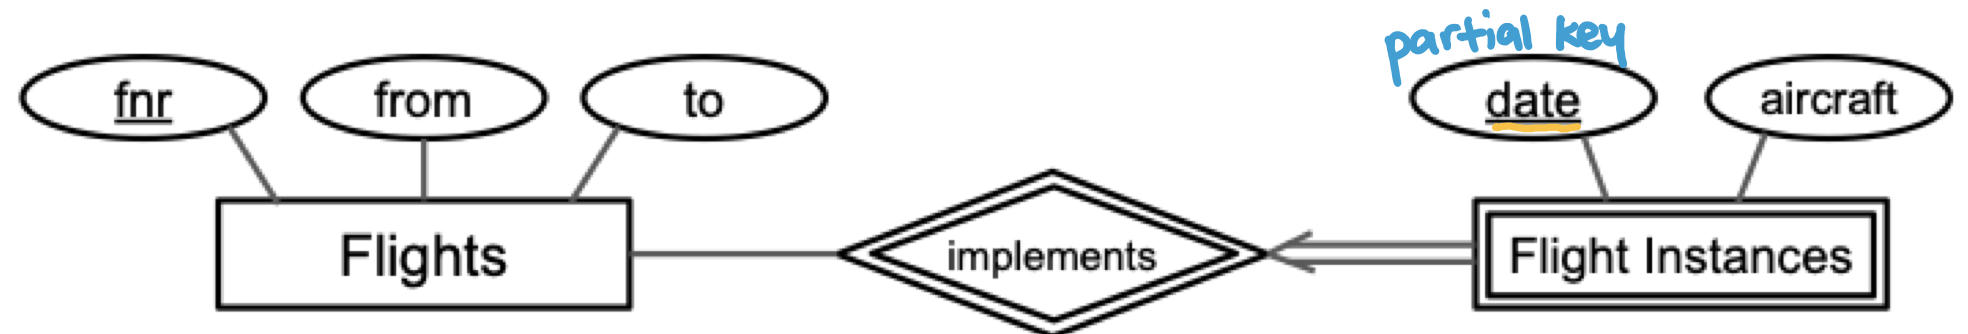
\includegraphics[width=0.95\linewidth]{cs2102-weak-entity-partial-key.png} 
      \end{itemize}
    \item requirements
      \begin{enumerate}
        \item many-to-one relationship (identifying relationship) from weak entity set to owner entity set
        \item weak entity set must have \textbf{total participation} in identifying relationship
      \end{enumerate}
  \end{itemize}

  \subsection{Participation Constraints}
  \begin{itemize}
    \item \definition{partial participation constraint} participation (of an entity in a relationship) is not mandatory (0 or more)
    \item \definition{total participation constraint} participation is mandatory (1 or more)
  \end{itemize}
  \begin{center}
    \begin{multicols}{2}
      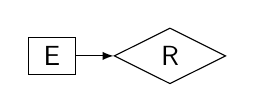
\begin{tikzpicture}
        \node[rectangle, draw, minimum width = 0.6cm] (e) at (0,0) {E};
        \node[diamond, draw, aspect = 2] (r) at (1.5,0) {R};
        \draw[-latex] (e) -- (r);
      \end{tikzpicture}
      \\* each instance of E participates 
      \\* in \textbf{at most one} instance of R

      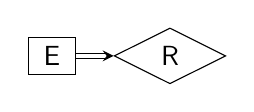
\begin{tikzpicture}
        \node[rectangle, draw, minimum width = 0.6cm] (e) at (0,0) {E};
        \node[diamond, draw, aspect = 2] (r) at (1.5,0) {R};
        \draw[-stealth, double, double distance = 1.2pt] (e) -- (r);
      \end{tikzpicture}
      \\* each instance of E participates 
      \\* in \textbf{exactly one} instance of R
      \\* \ 

      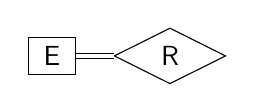
\begin{tikzpicture}
        \node[rectangle, draw, minimum width = 0.6cm] (e) at (0,0) {E};
        \node[diamond, draw, aspect = 2] (r) at (1.5,0) {R};
        \draw[double, double distance=1.2pt] (e) -- (r);
      \end{tikzpicture}
      \\* each instance of E participates 
      \\* in \textbf{at least one} instance of R
      \\ \ 

      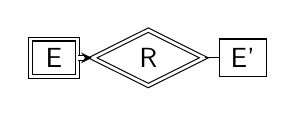
\begin{tikzpicture}
        \node[rectangle, double, draw, minimum width = 0.6cm, double distance=1pt] (e) at (0,0) {E};
        \node[diamond, double, draw, aspect = 2, double distance=1pt] (r) at (1.2,0) {R};
        \node[rectangle, draw, minimum width = 0.6cm] (e2) at (2.4,0) {E'};
        \draw[-stealth, double, double distance=1.2pt] (e) -- (r);
        \draw[-] (r) -- (e2);
      \end{tikzpicture}
      \\* E is a \textbf{weak entity set} 
      with identifying owner E' 
      \& identifying relationship set R.
    \end{multicols}
  \end{center}

  \subsection{Cardinality Constraints}
  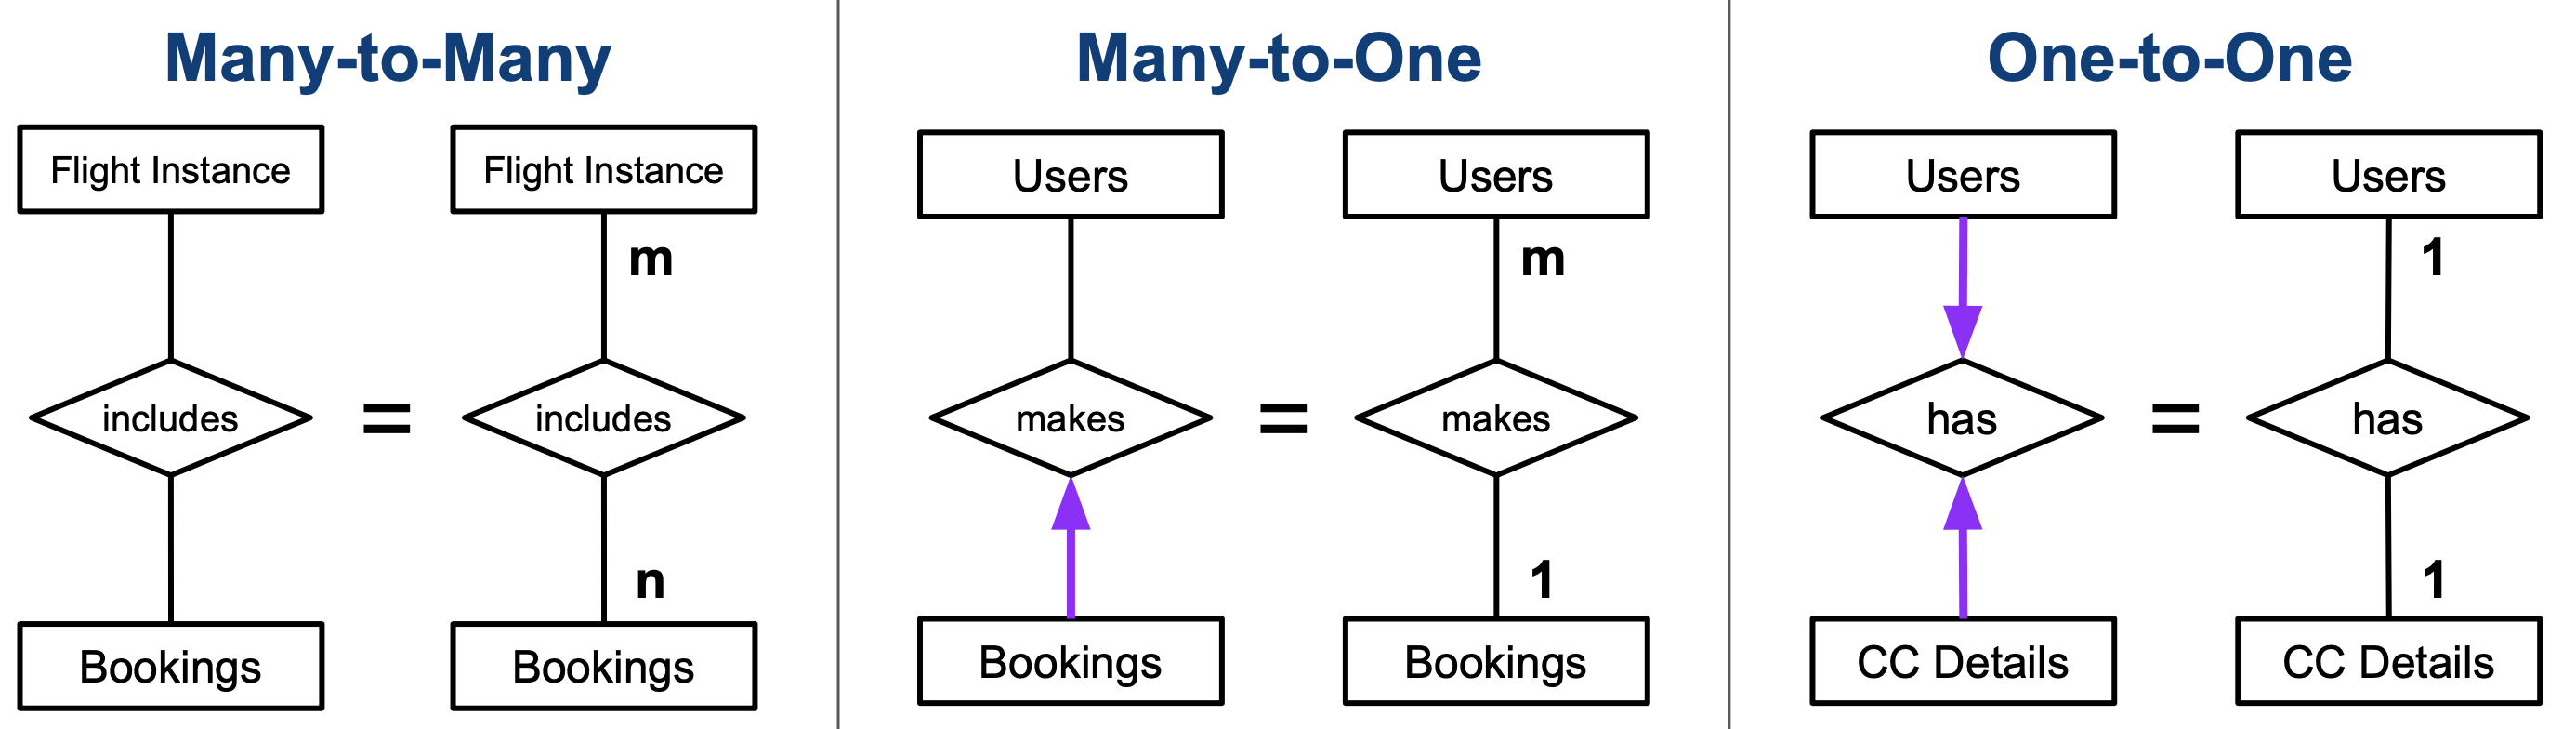
\includegraphics[width=0.95\linewidth]{cs2102-alternative-representation-cardinality-constraint.png} 

  \subsection{Alternative Representations}
  \begin{tightcenter}
    \begin{minipage}[c]{0.35\linewidth}
      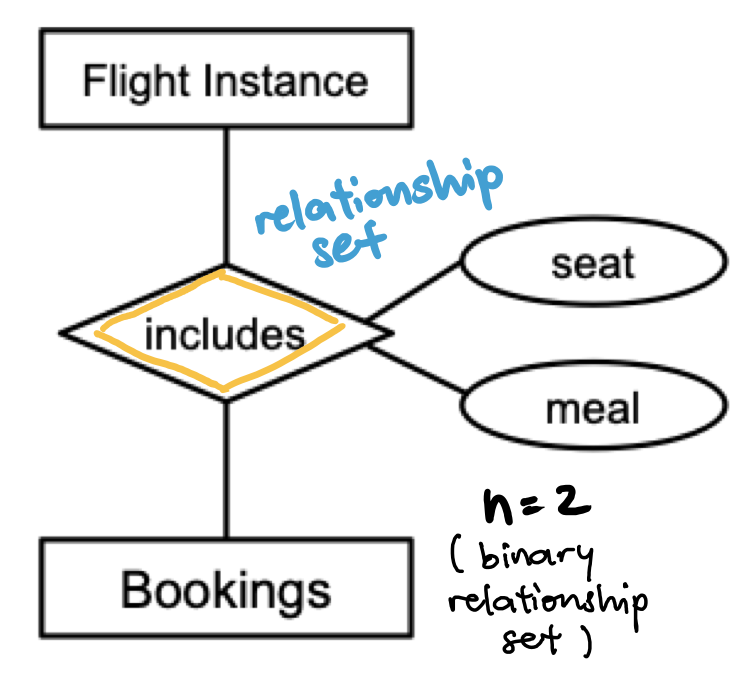
\includegraphics[width=0.95\linewidth]{cs2102-relationship-set.png} 
    \end{minipage}
    \begin{minipage}[c]{0.6\linewidth}
      \textbf{Min/Max notation}
      \\* 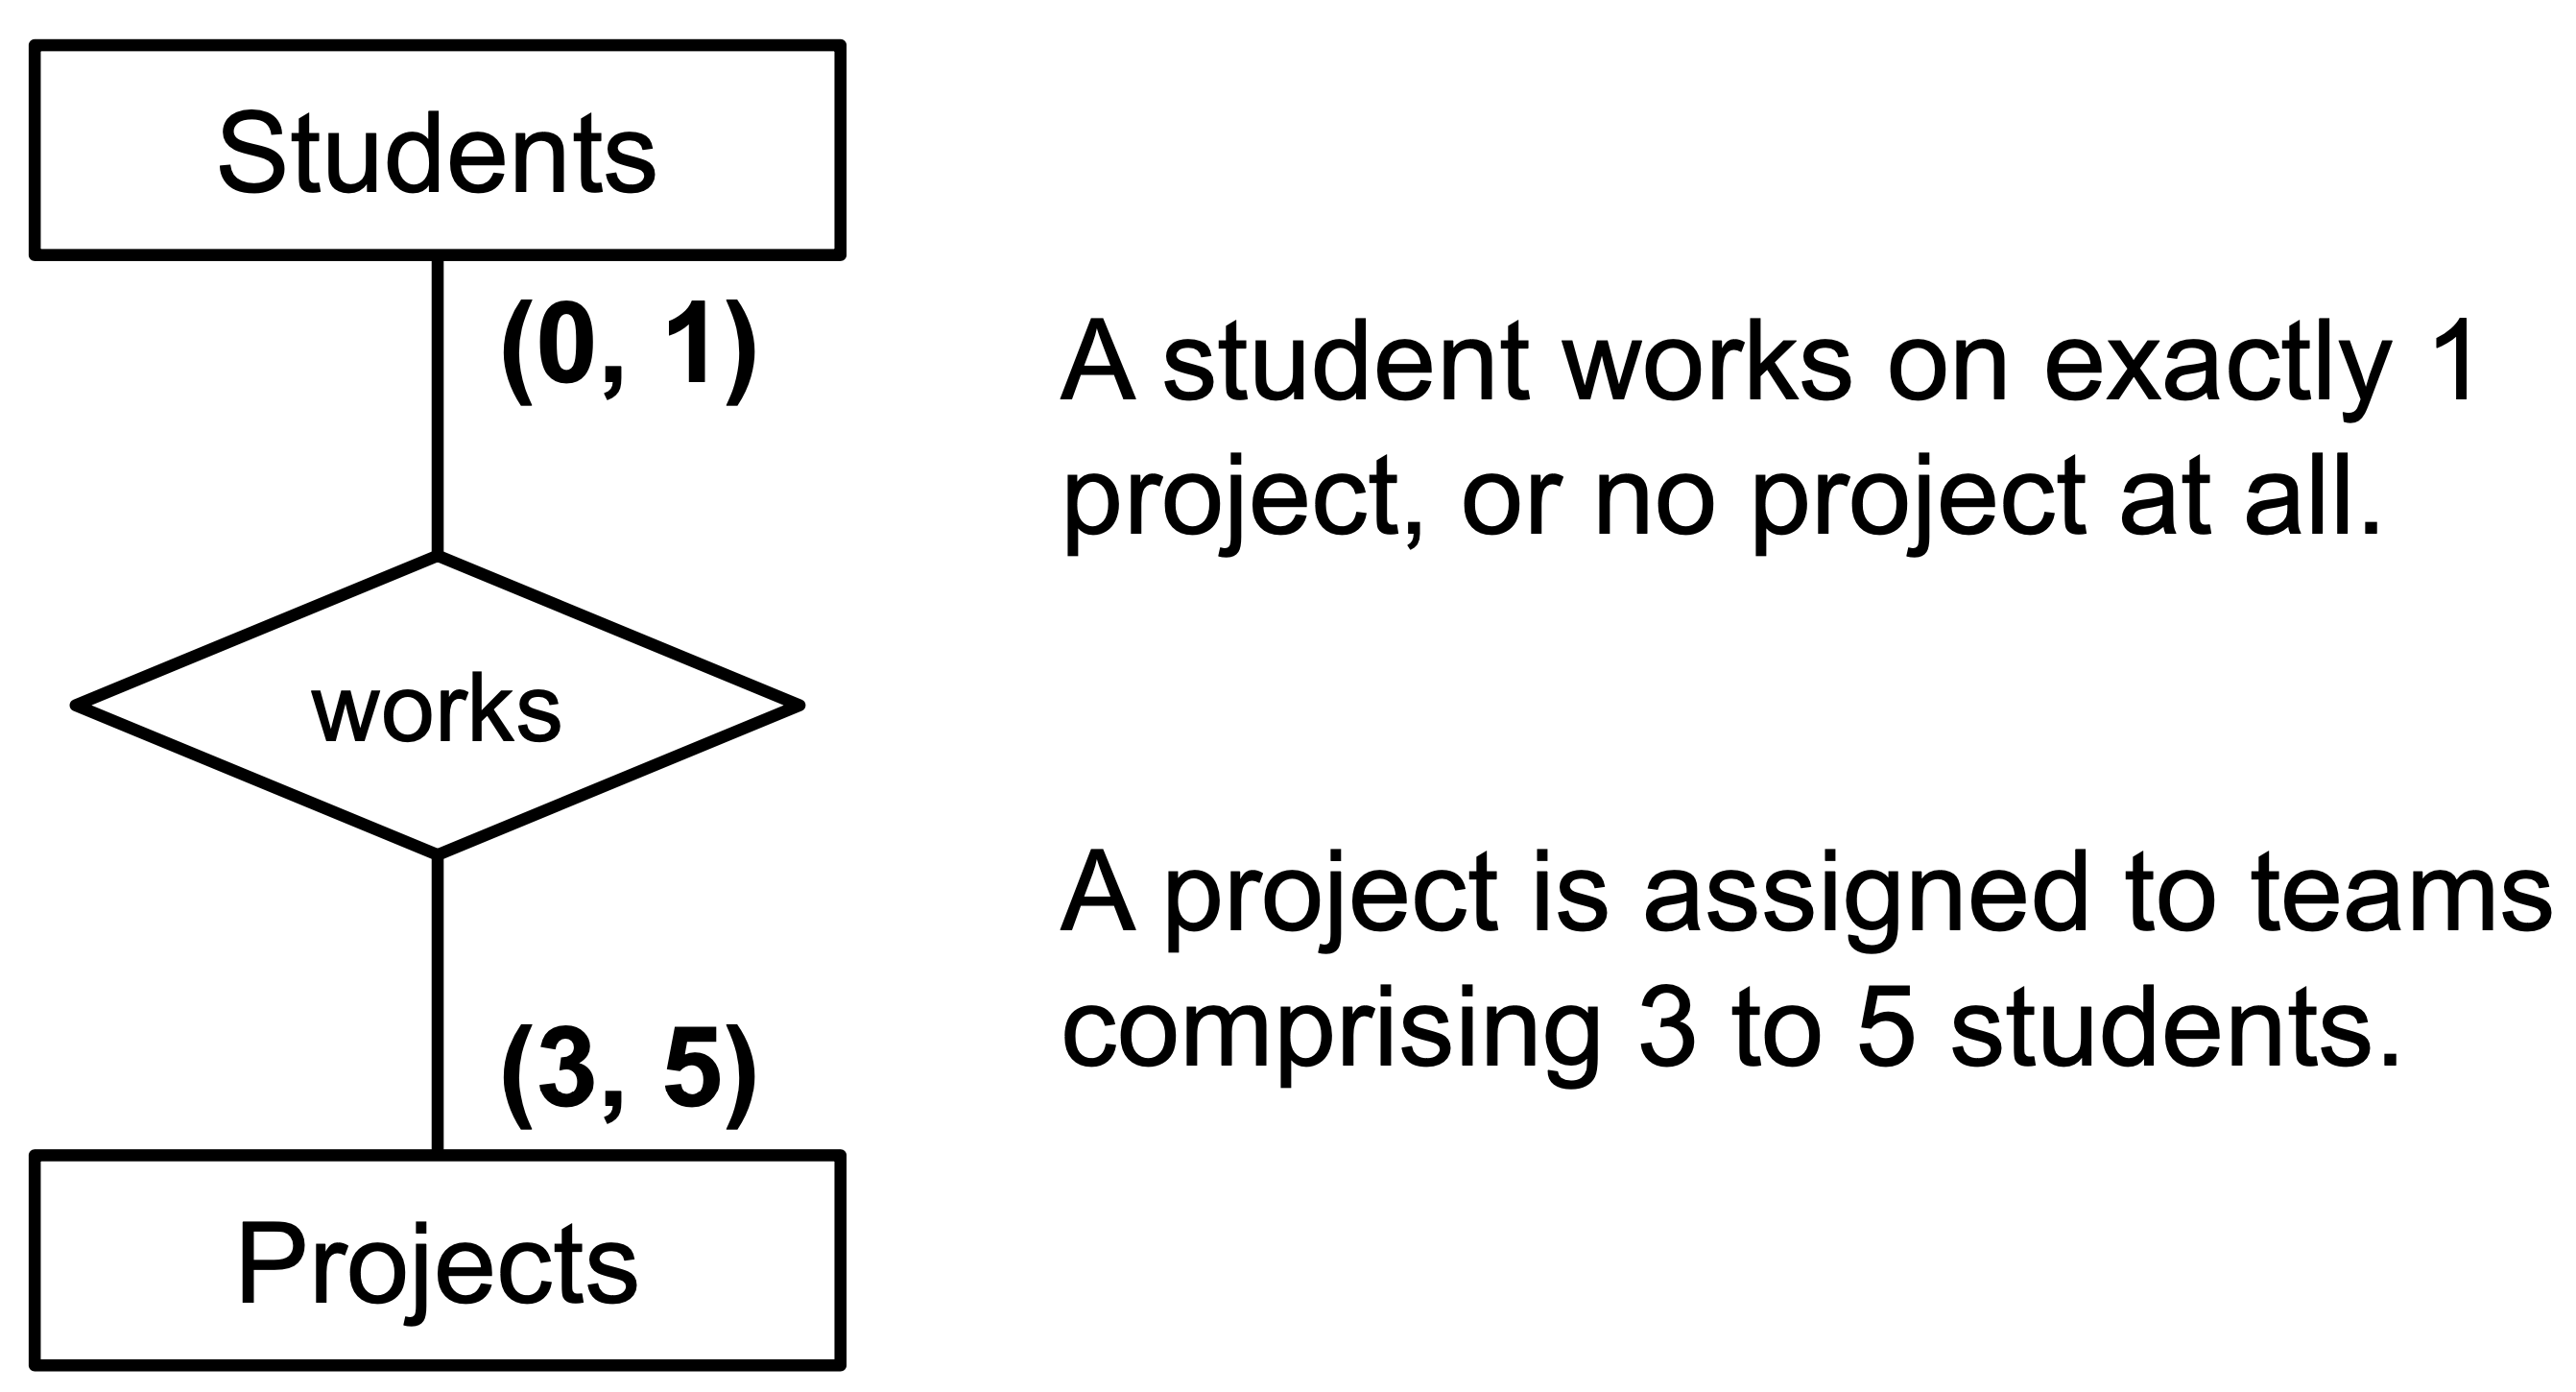
\includegraphics[width=0.9\linewidth]{cs2102-alternative-representation-minmax.png} 
    \end{minipage}
  \end{tightcenter}

  \subsection{ISA Hierarchy Constraints}
  \begin{itemize}
    \item \definition{overlap contraint} a superclass entity can belong to \textbf{multiple} subclasses
    \item \definition{covering constraint} a superclass entity \textbf{has to} belong to a subclass
  \end{itemize}
  \begin{tightcenter}
    \begin{minipage}[c]{0.55\linewidth}
      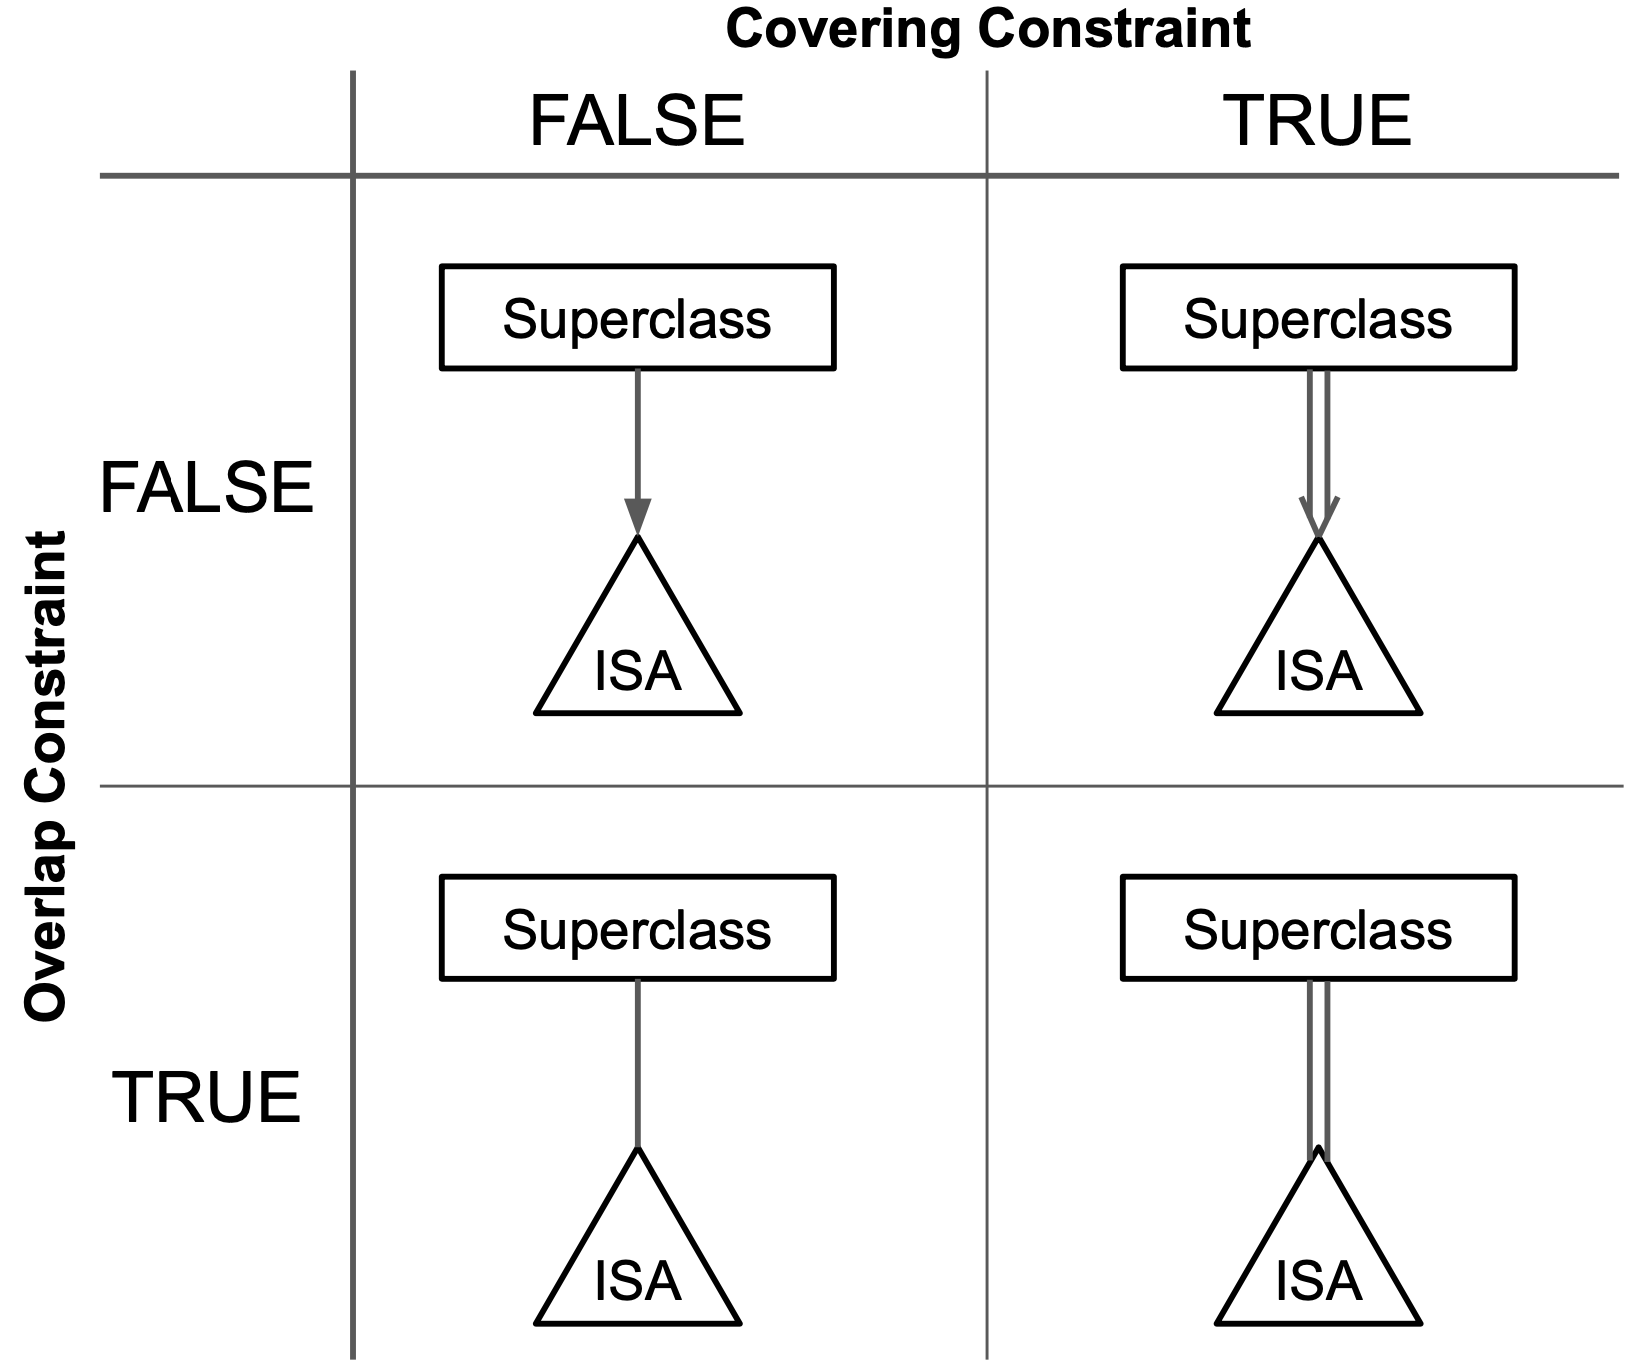
\includegraphics[width=0.95\linewidth]{cs2102-isa-hierarchy-notations.png} 
    \end{minipage}
    \begin{minipage}[c]{0.4\linewidth}
      \scriptsize superclass belongs to: \\
      \begin{tabular}{|c|c|c|}
        \hline
        & \scriptsize{F} & \scriptsize T \\ \hline
        \scriptsize F & \tiny\makecell{at most \\ one} & \tiny\makecell{exactly \\ one} \\ \hline
        \scriptsize T & \tiny\makecell{any \\ number of} & \tiny\makecell{at least \\ one} \\ \hline
      \end{tabular}
      \\ \scriptsize ... subclass
    \end{minipage}
  \end{tightcenter}

  \subsection{Aggregation}
  \begin{itemize}
    \item abstraction that treats \textbf{relationships} as higher-level entities
      \begin{itemize}
        \item e.g. treating 2 entities + 1 relationship as an entity set
      \end{itemize}
  \end{itemize}
  \begin{minipage}[c]{0.58\linewidth}
    \begin{lstlisting}[style=mySQL, basicstyle=\tiny]
CREATE TABLE Uses (
  gid INTEGER,
  sid CHAR(20),
  pname VARCHAR(50),
  hours NUMERIC,
  PRIMARY KEY (gid, sid, pname),
  FOREIGN KEY (gid) REFERENCES GPUs (gid),
  FOREIGN KEY (sid, pname) REFERENCES works (sid, pname)
);
    \end{lstlisting}
  \end{minipage}
  \begin{minipage}[c]{0.4\linewidth}
    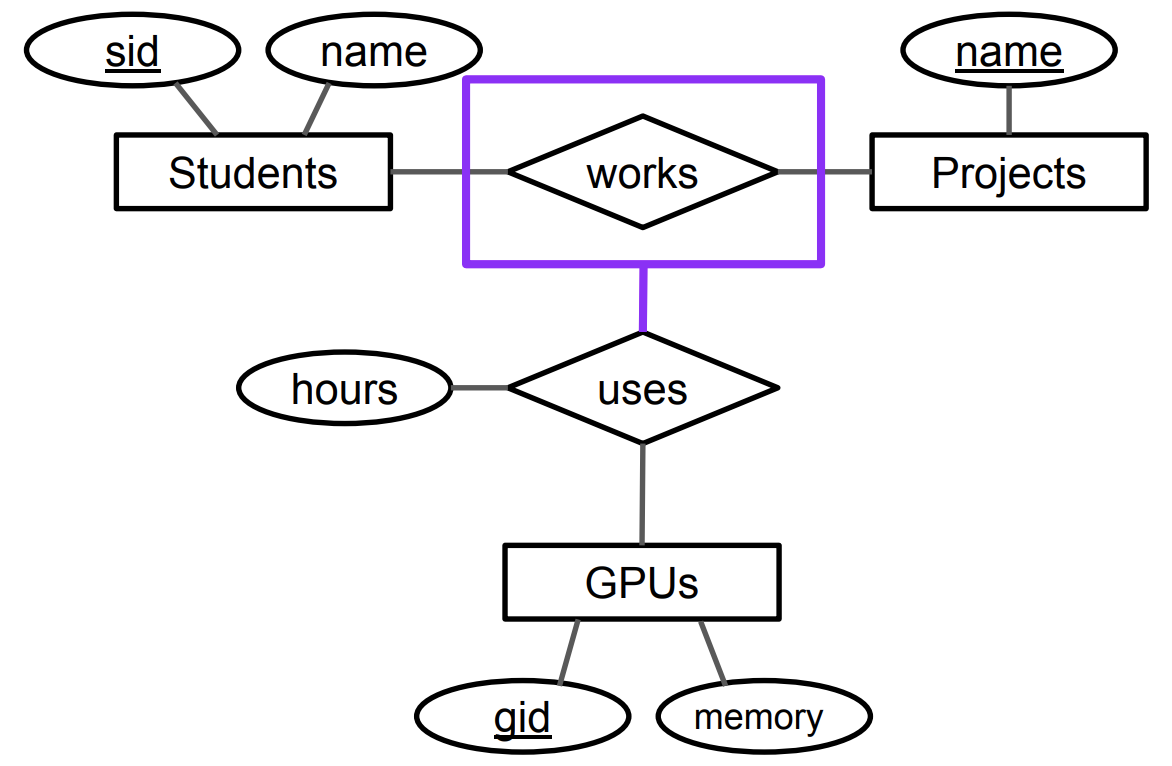
\includegraphics[width=0.98\linewidth]{cs2102-aggregation-example.png} 
  \end{minipage}

  \section{SQL}
  \begin{itemize}
    \item FROM $\rightarrow$ WHERE $\rightarrow$ GROUP BY $\rightarrow$ HAVING $\rightarrow$ SELECT $\rightarrow$ ORDER BY $\rightarrow$ LIMIT/OFFSET
    \item \code{\_} - any single character; \code{\%} - any sequence of characters (*)
    \item \code{UNION}/\code{INTERSECT}/\code{EXCEPT}: removes duplicate tuples
    \item \code{UNION ALL}/\code{... ALL}: keeps duplicates
    \item if column $A_i$ or table $R$ appears in the \code{SELECT}/\code{HAVING} clause, one of the following conditions must hold:
      \begin{enumerate}
        \item $A_i$ appears in the GROUP BY clause
        \item $A_i$ appears as input of an aggregation function in the SELECT clause
        \item the primary key of $R$ appears in the GROUP BY clause
      \end{enumerate}
    \item \textbf{\code{NULLIF(val1, val2)}} returns val1 == val2 ? \code{null} : \code{val1}
  \end{itemize}

  \subsection{Handling NULLs}
  \begin{itemize}
    \item \textbf{comparison} operation with \code{null} $\Rightarrow$ \textit{unknown}
    \item \textbf{arithmetic} operation with \code{null} $\Rightarrow$ \code{null}
    \item \code{null = null} $\Rightarrow$ \textit{unknown} (null, neither true nor false)
    \item \code{null = some\_value} $\Rightarrow$ neither true nor false
  \end{itemize}
  \begin{tightcenter}
    \scriptsize{\rowcolors{2}{gray!15}{gray!5}\begin{tabular}
        {ccccc}
        \rowcolor{cyan!10} 
        \textbf{x} & \textbf{y} & x<>y & x IS DISTINCT FROM y & x IS NULL \\ \hline 
        1 & 1 & FALSE & FALSE & FALSE \\ 
        1 & 2 & TRUE & TRUE & FALSE \\
        \textit{null} & 1 & \textit{null} & TRUE & TRUE \\
        \textit{null} & \textit{null} & \textit{null} & FALSE & TRUE \\
        \hline
      \end{tabular}
    }
    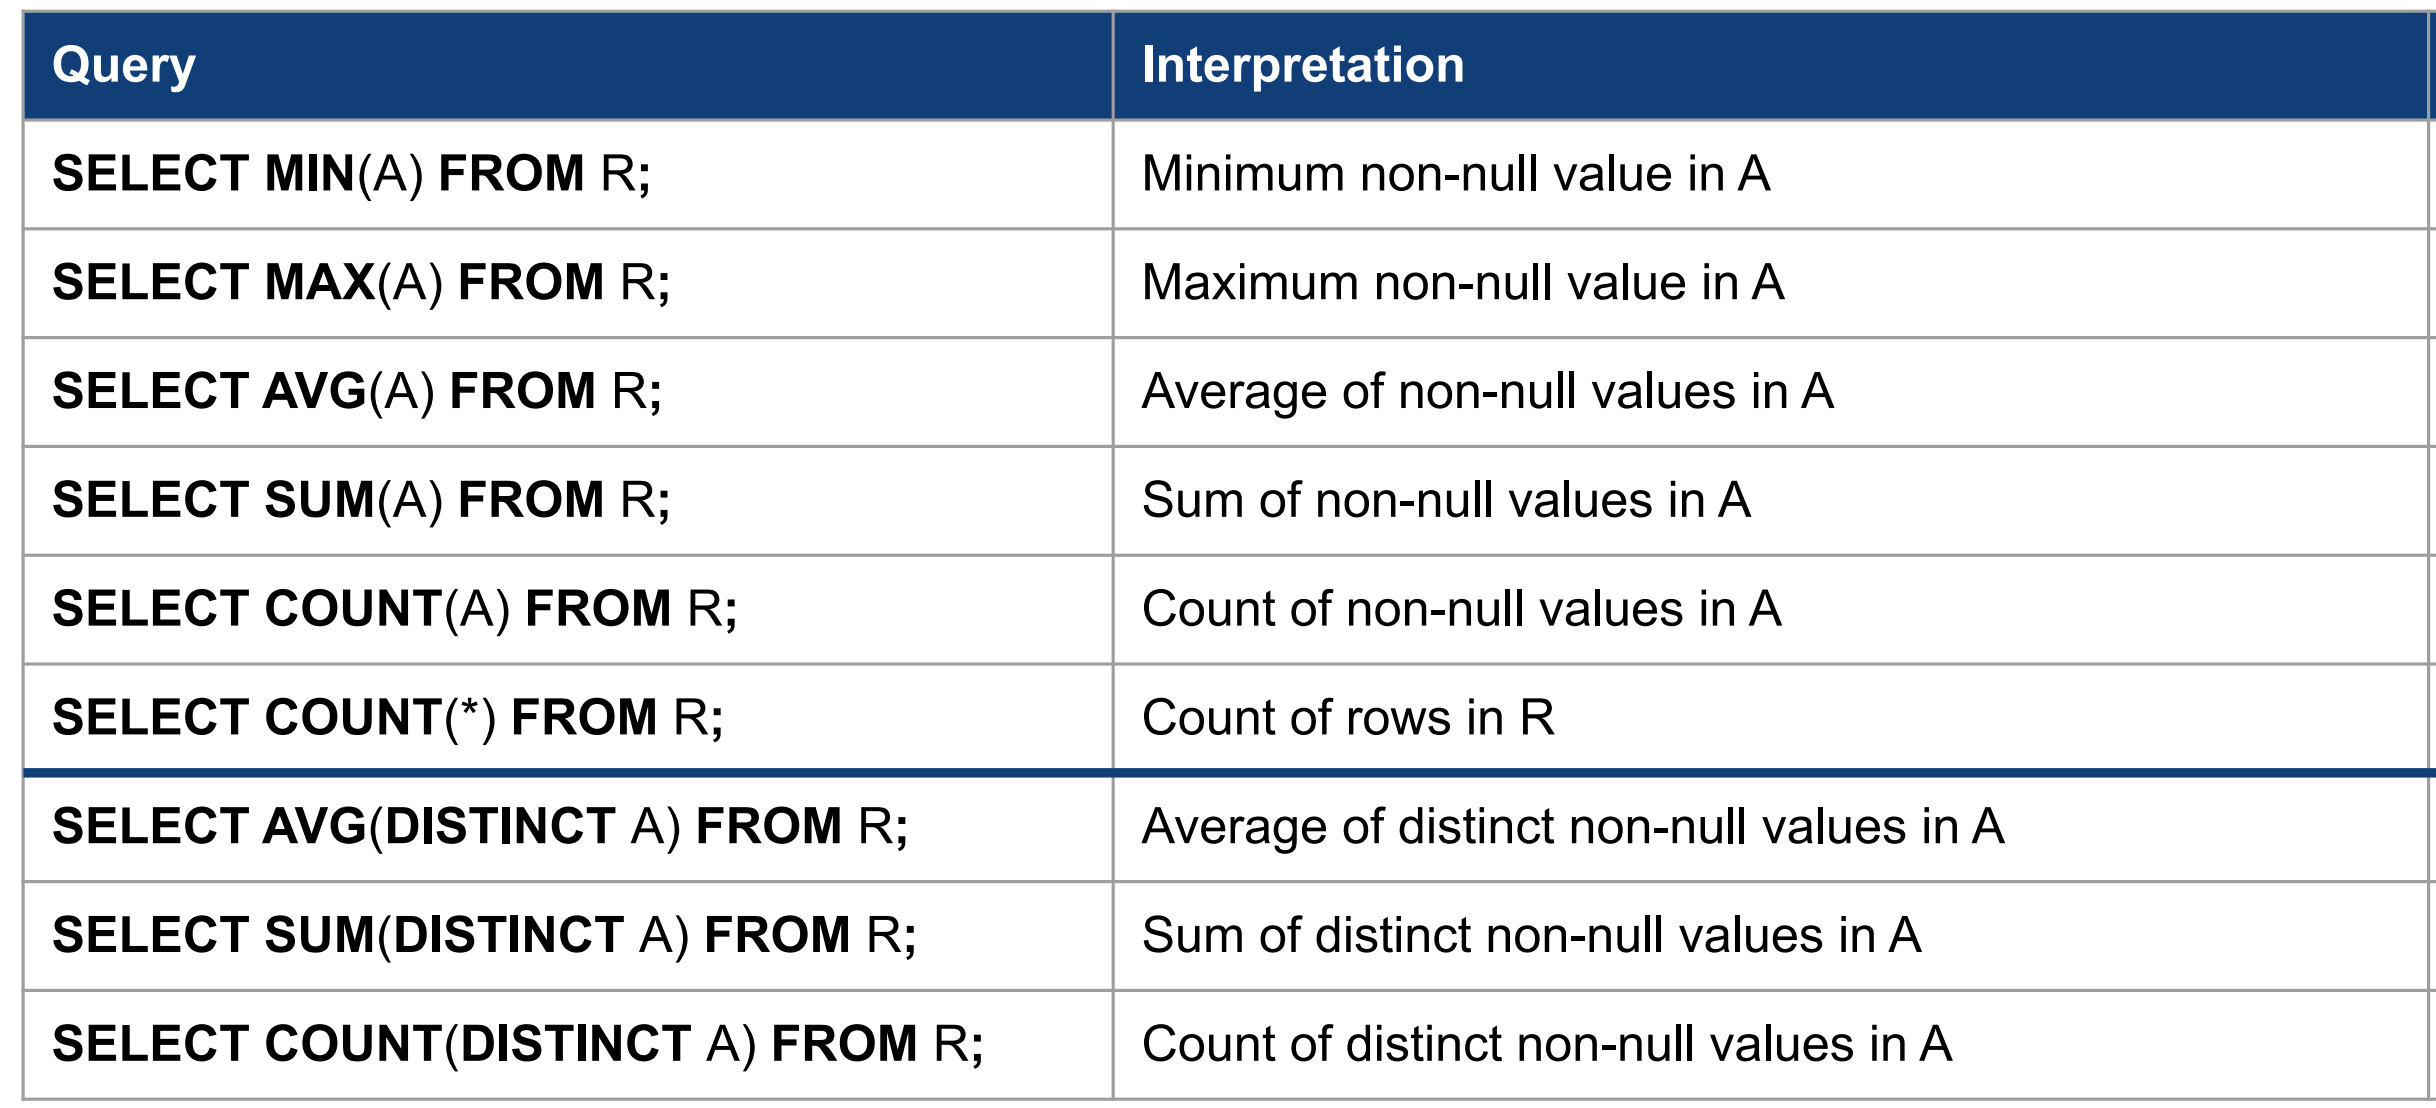
\includegraphics[width=0.95\linewidth]{cs2102-aggregation-functions-summary.png} 
    \\ Let $R$ be an empty relation; let $S$ be a non-empty relation with $n$ tuples but ONLY null values for $A$.
    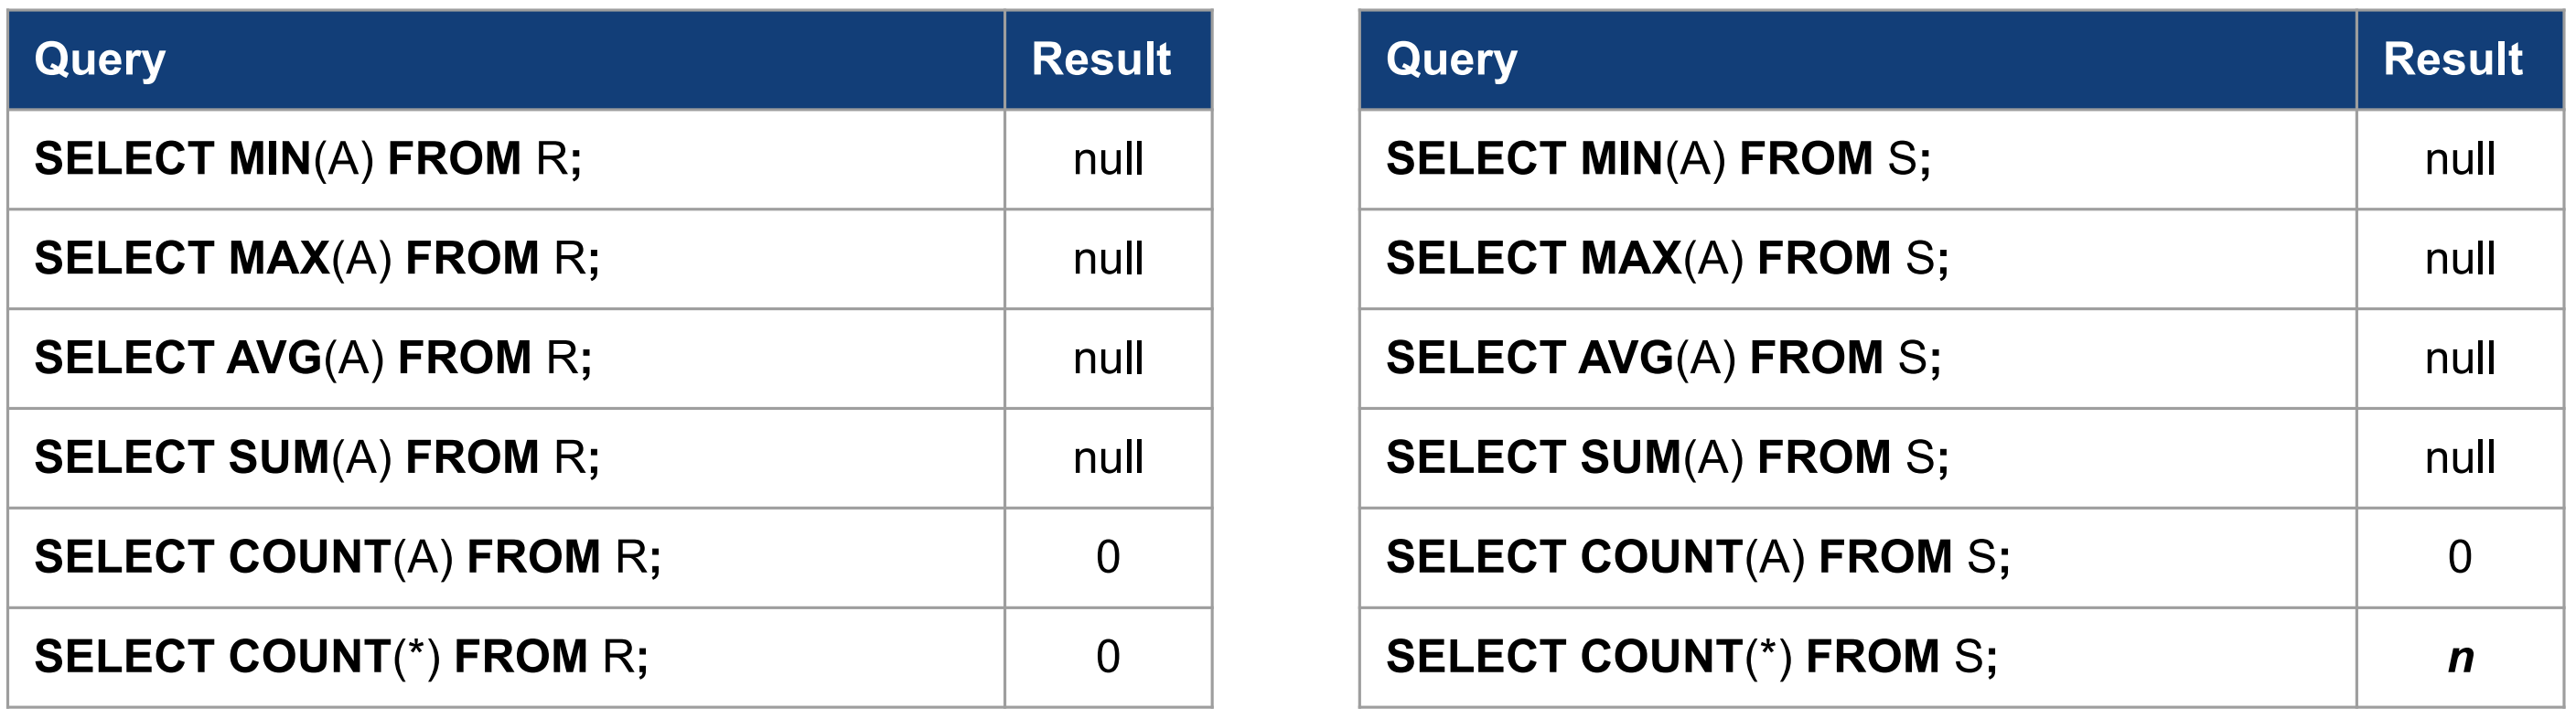
\includegraphics[width=0.95\linewidth]{cs2102-aggregation-function-null.png} 
  \end{tightcenter}


  \section{RELATIONAL ALGEBRA}

  \subsection{UNARY OPERATORS}
  \subsubsection{Selection, $ \sigma_c $}
  \begin{itemize}
    \item \definition{$\sigma_c(R)$} select all tuples from $ R $ satisfying condition $ c $.
      \begin{itemize}
        \item $\forall$ tuple $ t \in R$, $\; t \in \sigma_c(R) \iff c $ evaluates true on $ t $ 
        \item input and output relation have the same schema
      \end{itemize}
    \item \definition{selection condition} 
      \begin{itemize}
        \item a \textit{boolean expression} of one of the following forms:
          \begin{itemize}
            \item constant selection - attribute \textbf{op} constant
            \item attribute selection - attribute$_1$ \textbf{op} attribute$_2$
            \item expr$_1 \land $ expr$ _2 ; \quad$ expr$_1 \lor $ expr$ _2 ; \quad \lnot $ expr $ ; \quad $(expr)
          \end{itemize}
        \item with \textbf{op} $\in \{=, <>, <, \leq, \geq, >\}$
          \begin{itemize}
            \item \textbf{operator precedence}: (), \textbf{op}, $\lnot$, $\land$, $\lor$
          \end{itemize}
      \end{itemize}
  \end{itemize}

  \subsubsection{Projection, $\pi_\ell$}
  \begin{itemize}
    \item \definition{$\pi_\ell(R)$} projects all attributes of a given \textbf{relation}  specified in list $\ell$ (duplicates removed from output relation)
      \begin{itemize}
        \item \textbf{order} of attributes matters!
      \end{itemize}
  \end{itemize}

  \subsubsection{Renaming, $\rho_\ell$}
  \begin{itemize}
    \item \definition{$\rho_\ell(R)$} renames the attributes of a relation  $R$ (with schema $R(A_1, A_2, \dots, A_n)$ )
    \item 2 possible formats for $\ell$
      \begin{itemize}
        \item $\ell$ is the new \textit{schema} in terms of the new attribute names
          \begin{itemize}
            \item $\ell = (B_1, B_2, \dots, B_n)$ 
            \item $B_i = A_i$ if attribute $A_i$ does not get renamed
          \end{itemize}
        \item $\ell$ is a list of attribute renamings of the form: $B_i \leftarrow A_i, \dots, B_k \leftarrow A_k$
          \begin{itemize}
            \item each $B_j \leftarrow A_j$ renames attribute $A_j$ to attribute $B_j$
            \item order of renaming doesn't matter
          \end{itemize}
      \end{itemize}
  \end{itemize}

  \subsection{SET OPERATORS}
  \begin{itemize}
    \item \definition{union} $R \cup S$ returns a relation w/ all tuples in both $R$ \textbf{or}  $S$
    \item \definition{intersection} $R \cap S$ ... all tuples in both $R$ \textbf{and}  $S$ 
    \item \definition{set difference} $R - S$ ... all the tuples in  $R$ \textbf{but not in}  $S$
  \end{itemize}
  \attention for all set operators: $R$ and $S$ must be \textbf{union-compatible} 

  \subsubsection{Union Compatibility}
  \begin{itemize}
    \item two relations $R$ and $S$ are \definition{union-compatible} if
      \begin{itemize}
        \item $R$ and $S$ have the same number of attributes; and
        \item corresponding attributes have the \textit{same or compatible domains} 
      \end{itemize}
    \item note: $R$ and $S$ do not have to use the same attribute names
  \end{itemize}

  \subsection{CROSS PRODUCT}
  \begin{itemize}
    \item \definition{cross product} given two relations $R(A, B, C)$ and $S(X, Y)$, $R \times S$ returns a relation with schema $(A, B, C, X, Y)$ defined as 
      \\* $R \times S = \{(a, b, c, x, y) \mid (a, b, c) \in R, (x, y) \in S\}$
    \item \textbf{size} of cross product $= \abs{R}*\abs{S}$
  \end{itemize}

  \section{JOIN OPERATORS}

  \subsection{Inner Joins} 
  \begin{itemize}
    \item eliminate all tuples that do not satisfy a matching criteria (i.e. \textbf{attribute selection})
    \item \definition{$\theta$-join} (of two relations $R$ and $S$) \( {\displaystyle{R \bowtie_\theta S = \sigma_\theta(R \times S)}} \) 
    \item \definition{Equi Join $\Join$} special case of $\theta$-join defined over the  \textbf{equality} operator ($=$) only
    \item \definition{Natural Join $\Join$} performed over all attributes $R$ and $S$ have in common
      \begin{itemize}
        \item the natural join (of two relations $R$ and $S$) is defined as 
          \\* $R \Join S = \pi_\ell(R\Join_c \rho_{b_i \leftarrow a_i, \dots, b_k \leftarrow a_k}(S))$
          \begin{itemize}
            \item $A=\{a_i, \dots, a_k\} =$ the set of attributes that $R$ and $S$ have in common
            \item $c = ((a_i = b_i) \land \dots \land (a_k = b_k))$
            \item $\ell =$ list of all attributes of $R$ + list of all attributes in $S$ that are \textbf{not in}  $A$
          \end{itemize}
        \item output relation contains the common attributes of $R$ and $S$ only \textit{once} 
      \end{itemize}
  \end{itemize}

  \subsection{Outer Joins}
  \begin{itemize}
    \item \definition{dangling tuples} tuples in $R$ or $S$ that do not match with tuples in the other relation
      \begin{itemize}
        \item \definition{$\textit{dangle}(R \Join_\theta S)$} set of dangling tuples in  $R$ wrt to $R \Join_\theta S$ (missing attribute values are padded with \code{null})
          \begin{itemize}
            \item $\textit{dangle}(R \Join_\theta S) \subseteq R$
          \end{itemize}
        \item always removed by inner joins, kept by outer joins
      \end{itemize}
    \item \definition{$null(R)$} $n$-component \textbf{tuple}  of \code{null} values where $n$ is the number of attributes of $R$
  \end{itemize}

  \subsubsection{Definitions}
  \begin{itemize}
    \item \definition{left outer join} $ R \lojoin_\theta S $
      \\* $= R \Join_\theta S \cup (\textit{dangle}(R \Join_\theta S) \times \{\textit{null}(S)\}) $
    \item \definition{right outer join} $ R \rojoin_\theta S $
      \\* $= R \Join_\theta S \cup (\{\textit{null}(R)\} \times \textit{dangle}(S \Join_\theta R))$
    \item \definition{full outer join} $R \fojoin_\theta S$ 
      \\* $= R \Join_\theta S \cup (\textit{dangle}(R \Join_\theta S) \times \{\textit{null}(S)\}) $ 
      $ \cup (\{\textit{null}(R)\} \times \textit{dangle}(S \Join_\theta R))$
  \end{itemize}

  \subsubsection{Natural Outer Joins}
  \begin{itemize}
    \item natural left/right/full outer join: $R \lojoin S$ / $R \rojoin S$ / $R \fojoin S$
    \item output relation contains the common attributes only once
  \end{itemize}


  \section{FUNCTIONAL DEPENDENCIES}

  \begin{itemize}
    \item \definition{normal form} a definition of minimum requirements in terms of \textbf{redundancy} 
    \item \definition{prime attribute} appears in at least one key
    \item an attribute not in any RHS of any FD \textbf{must} be in every key
  \end{itemize}

  \subsection{Functional Dependencies}
  Let $A_1, A_2, \dots, A_m, B_1, B_2, \dots, B_n$ be some attributes.
  \begin{itemize}
    \item \definition{uniquely identifies} $\{A_1 A_2 \dots A_m \} \rightarrow \{B_1 B_2 \dots B_n\}$ whenever 2 tuples have the same values on $A_1 A_2 \dots A_m$, they always have the same values on $B_1 B_2 \dots B_n$
      \begin{itemize}
        \item $\{A\} \rightarrow \{B\}$ : functional dependency - $A$ determines $B$ 
      \end{itemize}
    \item two \textbf{attributes} are \definition{functionally equivalent} if either one can determine the other
    \item \definition{dependency preserving} can derive all FDs from table closures
    \item \definition{equivalence} F1 is equivalent to F2 ($F1 \equiv F2$) $\Leftrightarrow$ 
      \begin{itemize}
        \item $F2 \vdash F1$: every FD in F1 can be derived from F2
        \item $F1 \dashv F2$: every FD in F2 can be derived from F1 
      \end{itemize}
  \end{itemize}

  \subsubsection{Armstrong's Axioms}
  \begin{enumerate}
    \item axiom of \textbf{reflexivity}: set $\rightarrow$ a subset of attributes 
      \\* ($\{A, B\} \rightarrow \{A\}$)
    \item axiom of \textbf{augmentation}: 
      \\* if $\{A\} \rightarrow \{B\}$, then $\forall C, \, \{AC\} \rightarrow \{BC\}$
    \item axiom of \textbf{transitivity}: 
      \\* if $\{A\} \rightarrow \{B\}$ and $\{B\} \rightarrow \{C\}$, then $\{A\} \rightarrow \{C\}$
  \end{enumerate}

  \textbf{Extended Armstrong's Axioms}
  \begin{itemize}
    \item rule of \textbf{decomposition}: 
      \\* if $\{A\} \rightarrow \{BC\}$ then $\{A\} \rightarrow \{B\} \land \{A\} \rightarrow \{C\}$
    \item rule of \textbf{union}: 
      \\* if $\{A\} \rightarrow \{B\} \land \{A\} \rightarrow \{C\}$, then $\{A\} \rightarrow \{BC\}$
    \item combined: $\{A\} \rightarrow \{BC\}$ $\Leftrightarrow$ $\{A\} \rightarrow \{B\} \land \{A\} \rightarrow \{C\}$
  \end{itemize}

  \subsection{Closures}
  \begin{itemize}
    \item $\{A_1A_2\dots A_m\}^+$ is the closure of $A_1A_2\dots A_m$  
  \end{itemize}


  \section{BOYCE-CODD NF (BCNF)}

  \subsection{BCNF}
  \begin{itemize}
    \item \definition{BCNF} every \textit{non-trivial \& decomposed FD} has a \textit{superkey} as its LHS
      \begin{itemize}
        \item stronger than 3NF - has fewer redundancies
      \end{itemize}

    \item \attention a table with exactly one or two attributes is always in BCNF!
    \item $\checkmark$ no update/deletion/insertion anomalies
    \item $\checkmark$ small redundancies
    \item $\checkmark$ \textbf{lossless join} - original table can always be reconstructed from decomposed tables (natural join). $\quad \Rightarrow \quad R = R1 \Join R2 = \pi_{R1}(R) \Join \pi_{R2}(R)$
    \item $\times$ may \textbf{not} preserve all FDs - decomposed table may have no non-trivial \& decomposed FDs
      \begin{itemize}
        \item exists FD that cannot be derived from FDs on R1 and R2
      \end{itemize}
    \item \definition{lossless decomposition} $\{R_1, R_2\}$ is lossless if $R_1 \cap R_2$ is a superkey of $R_1$ or $R_2$ 
      \begin{itemize}
        \item $R_1 \cap R_2$ uniquely identifies all the attributes in $R_1$ or $R_2$
        \item closure of $R_1 \cap R_2 = R_1$ or $R_2$ 
      \end{itemize}
  \end{itemize}

  \subsubsection{Non-Trivial and Decomposed FD}
  \begin{itemize}
    \item \definition{non-trivial} $\{A\} \rightarrow \{B\}$ where $\{B\} \not\subseteq \{A\}$
    \item \definition{decomposed} $\{A\} \rightarrow \{B\}$ where $B$ is a single attribute
  \end{itemize}

  \subsection{BCNF Normalisation}
  \begin{itemize}
    \item for a BCNF-violating FD $\{A\} \rightarrow \{A\}^+$, create tables
      \begin{itemize}
        \item $R1(\{A\}^+)$ containing the superkey, and 
        \item $R2 \left( \, \{A\} \cup (R - \{A\}^+) \, \right)$
      \end{itemize}
    \item if table does not contain all attributes:
      \begin{enumerate}
        \item compute closure of each subset of the table's attributes
        \item remove RHS attributes not in the table
      \end{enumerate}
  \end{itemize}

  \attention \textit{implicit} functional dependencies should be checked too! (because explicit FDs may not apply to R2 when R2 is missing attributes)

  \begin{tightcenter}
    \begin{minipage}[c]{0.47\linewidth}
      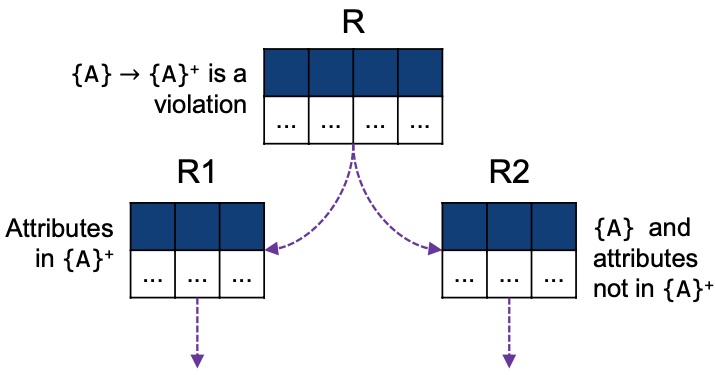
\includegraphics[width=0.95\linewidth]{cs2102-bcnf-decomposition.png} 
    \end{minipage}
    \begin{minipage}[c]{0.47\linewidth}
      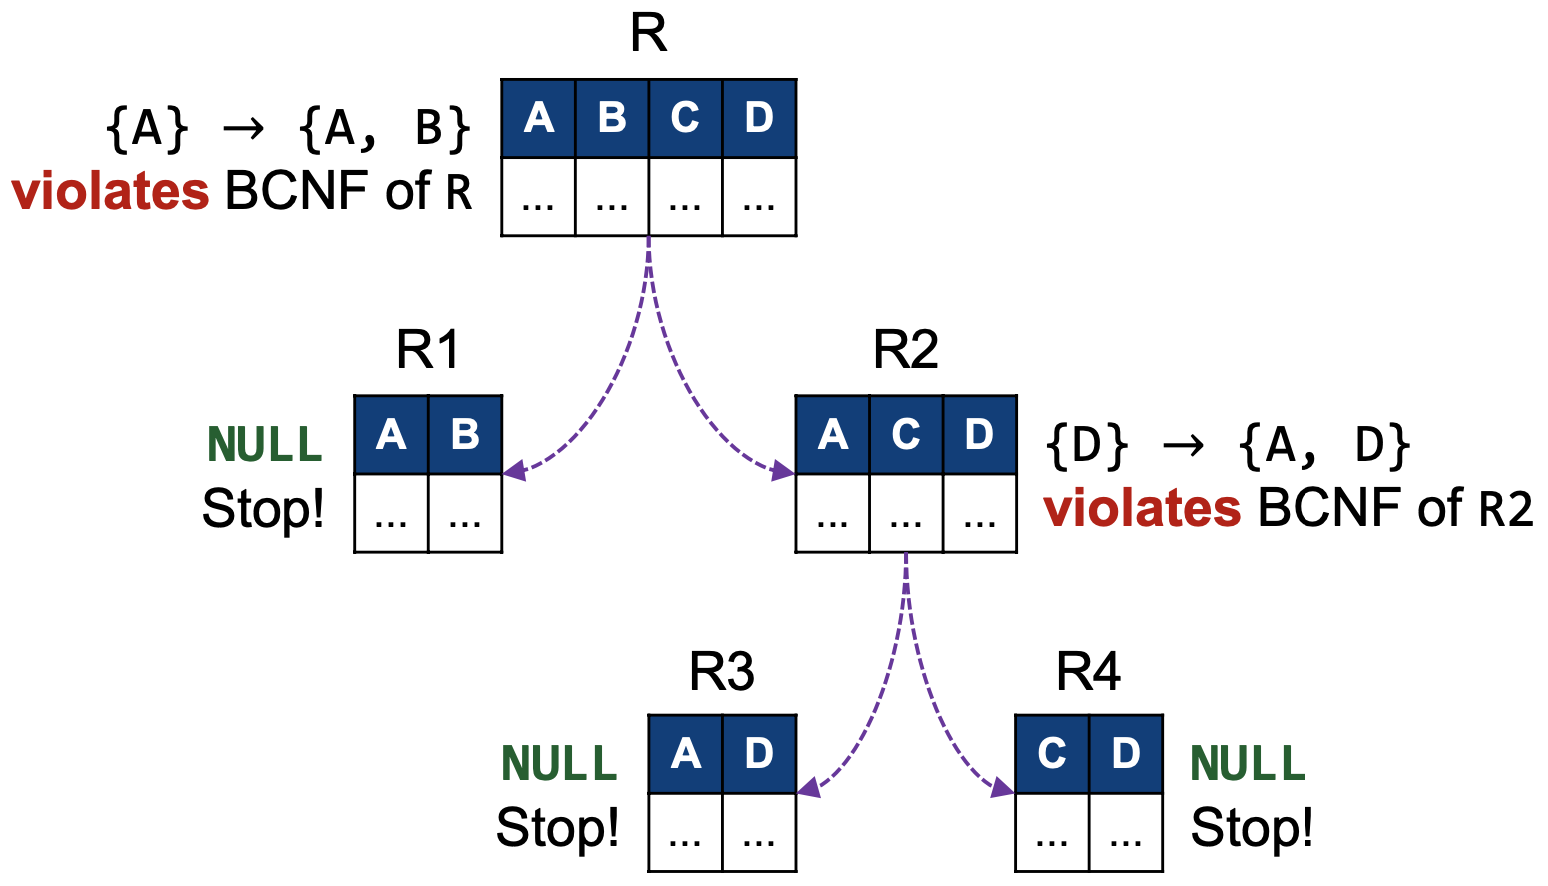
\includegraphics[width=0.95\linewidth]{cs2102-bcnf-decomposition-example.png} 
    \end{minipage}
    e.g. $R(A,B,C,D)$ with $BC \rightarrow D$, $D \rightarrow A$,  $A \rightarrow B$
  \end{tightcenter}

  \section{THIRD NORMAL FORM (3NF)}
  \subsection{3NF}
  \begin{itemize}
    \item a table is in \definition{3NF} if every \textit{non-trivial} \& \textit{decomposed} FD:
      \begin{itemize}
        \item its LHS is a \textbf{superkey}, OR
        \item its RHS is a \textbf{prime attribute} (any attribute in any key)
      \end{itemize}
    \item $\checkmark$ will preserve all FDs
    \item relaxed form of BCNF
      \begin{itemize}
        \item satisfies BCNF $\Rightarrow$ satisfies 3NF
        \item violates 3NF $\Rightarrow$ violates BCNF
      \end{itemize}
    \item if all attributes are prime attributes, the table is in 3NF
  \end{itemize}

  \subsection{3NF Synthesis}
  for table R and a set of FDs F,
  \begin{enumerate}
    \item derive \textit{minimal basis} $F_b$ of F
    \item from the minimal basis, combine (union) the FDs for which the LHS is the same (\textbf{canonical cover})
    \item create a table for each FDs remained in the minimal basis after union 
    \item if \textbf{none} of the tables contain a key for the original table R, create a table containing a key of R
  \end{enumerate}

  \subsection{Minimal Basis / Minimal Cover}
  \begin{itemize}
    \item minimal basis, $F_b$: \definition{simplified} 4 conditions
      \begin{enumerate}
        \item equivalence: $F \equiv F_b$ (every FD in $F_b$ can be derived from F and vice versa)
        \item every FD in $F_b$ is non-trivial and decomposed
        \item $\forall$ FD in $F_b$, none of the LHS attributes are redundant
        \item no FD in $F_b$ is redundant
      \end{enumerate}
    \item \definition{redundant} can be removed without affecting the original FD (i.e. $F \equiv F_{b*}$ where  $F_{b*}$ is formed by removing the attribute)
  \end{itemize}

  \subsubsection{to obtain a minimal basis}
  \begin{enumerate}
    \item ensure equivalence
    \item transform FDs to non-trivial and decomposed
    \item remove redundant attributes
      \begin{enumerate}
        \item for an FD \{A\} $\rightarrow$ B for a \textbf{set} of attributes A, for an attribute C in A,
        \item compute $\{A-C\}^+$ using F
        \item if $B \in \{A-C\}^+$, then we can remove C
      \end{enumerate}
    \item remove redundant FDs
      \begin{enumerate}
        \item try removing and check for equivalence
      \end{enumerate}
  \end{enumerate}

  \section{COMMON ER MODELS}
  \begin{tightcenter}
    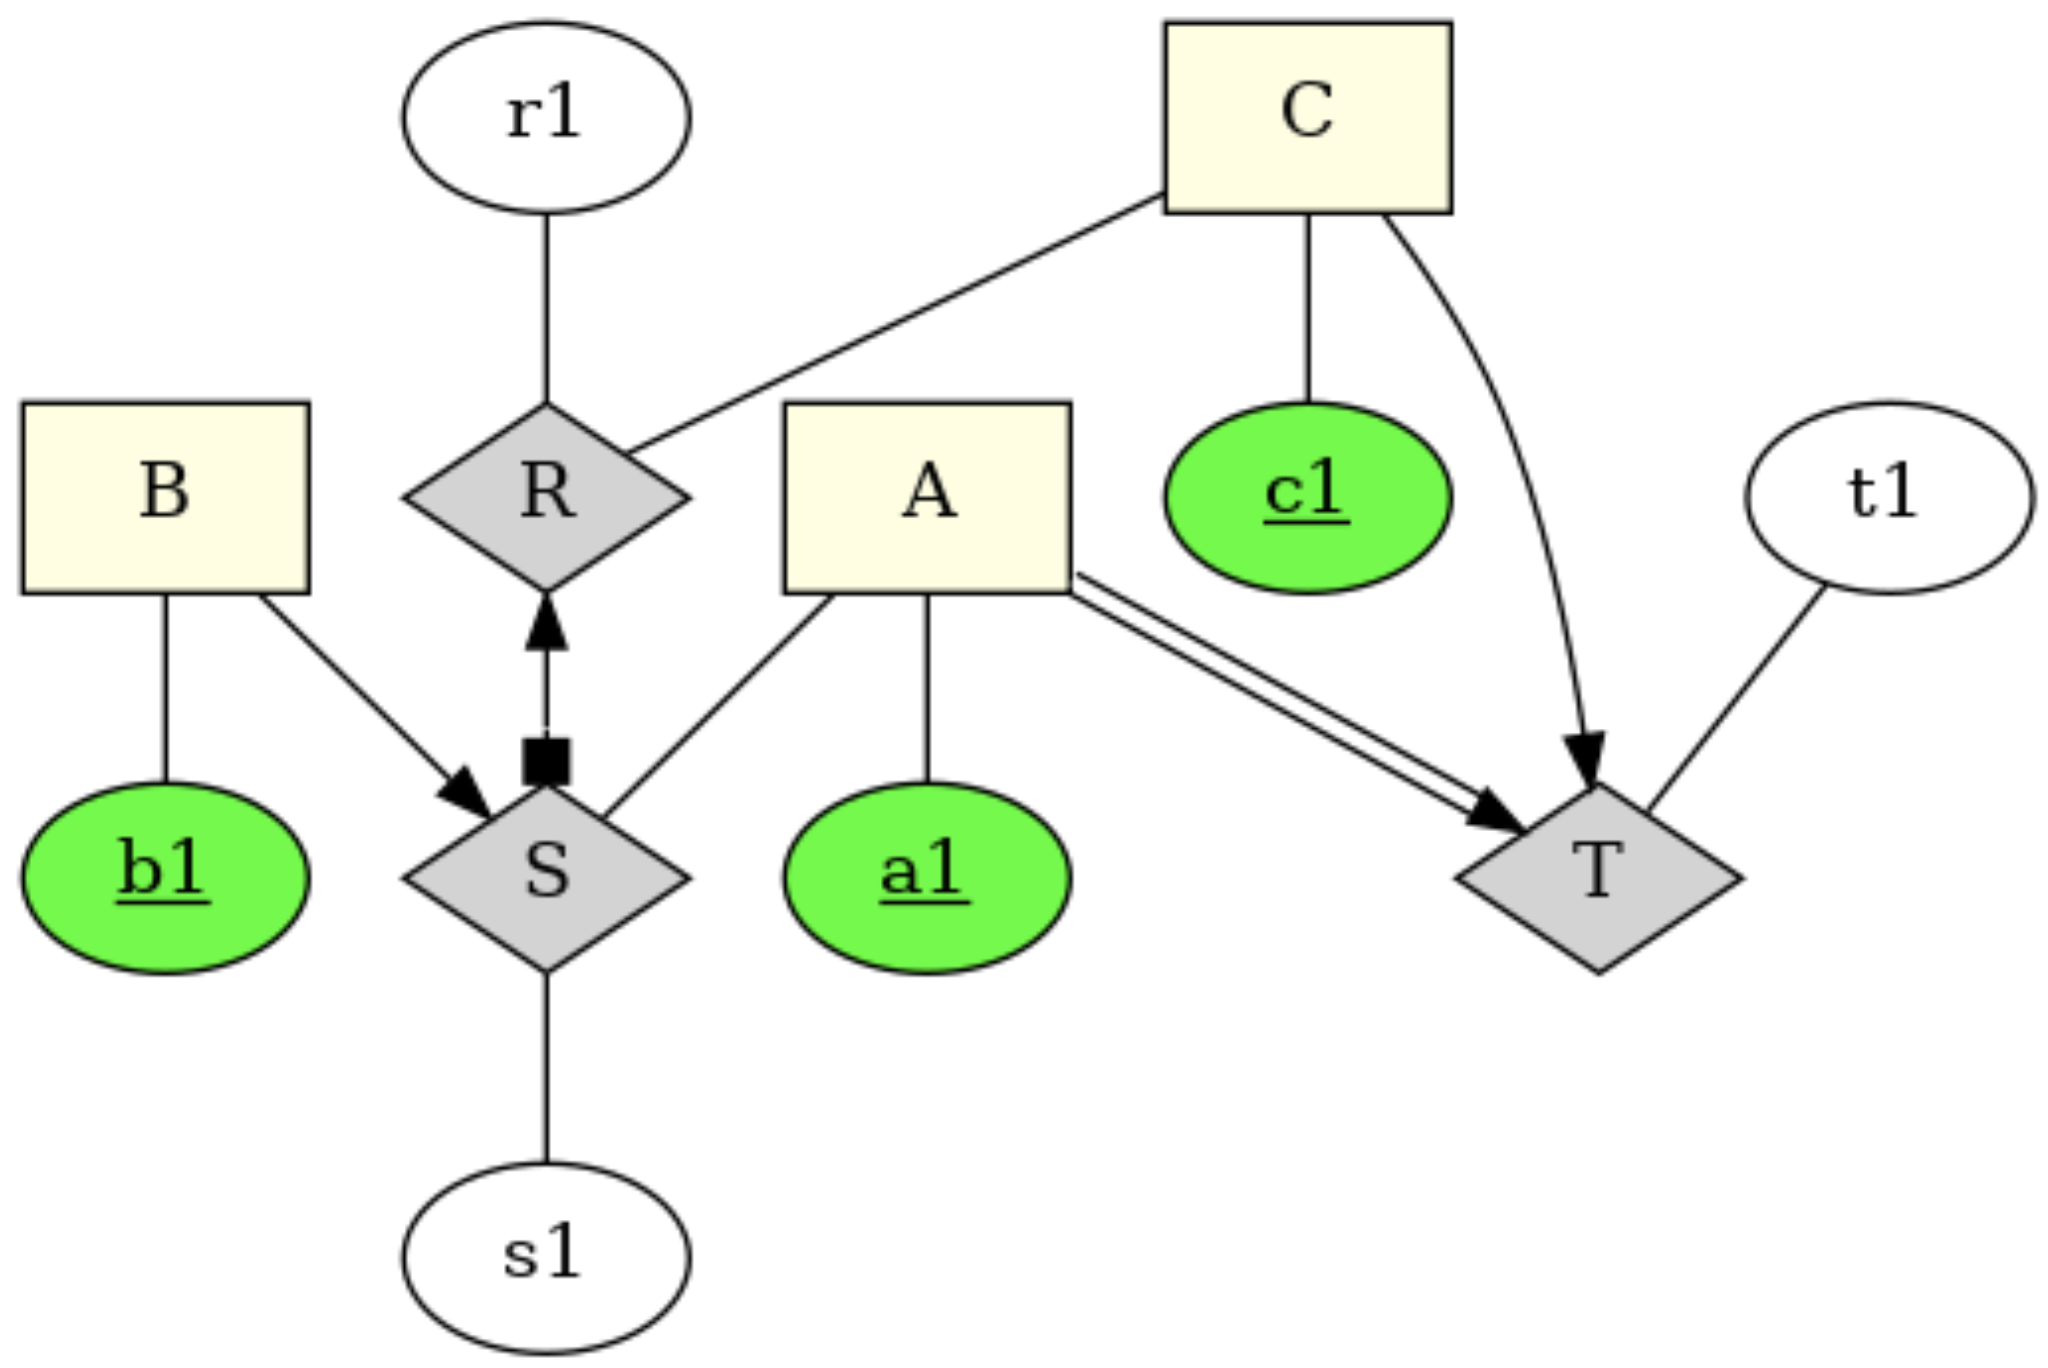
\includegraphics[width=0.8\linewidth]{cs2102-er-model-participation-constraints.png} 
  \end{tightcenter}
  \begin{minipage}[c]{0.45\linewidth}
    \begin{lstlisting}[style=mySQL, basicstyle=\tiny]
-- merge A and T
CREATE TABLE B (
  b1 	integer,
  PRIMARY KEY (b1)
);

CREATE TABLE C (
  c1 	integer,
  PRIMARY KEY (c1)
);

CREATE TABLE AT (
  a1 	integer,
  c1 	integer NOT NULL,
  t1 	integer NOT NULL,
  PRIMARY KEY (a1),
  UNIQUE (c1),
  FOREIGN KEY (c1) REFERENCES C
);

CREATE TABLE S (
  a1 	integer NOT NULL,
  b1 	integer,
  s1 	integer NOT NULL,
  PRIMARY KEY (b1),
  FOREIGN KEY (a1) REFERENCES AT,
  FOREIGN KEY (b1) REFERENCES B
);

CREATE TABLE R (
  b1 	integer,
  c1 	integer NOT NULL,
  r1 	integer NOT NULL,
  PRIMARY KEY (b1),
  FOREIGN KEY (c1) REFERENCES C,
  FOREIGN KEY (b1) REFERENCES S
);
    \end{lstlisting}
  \end{minipage}
  \begin{minipage}[c]{0.52\linewidth}
    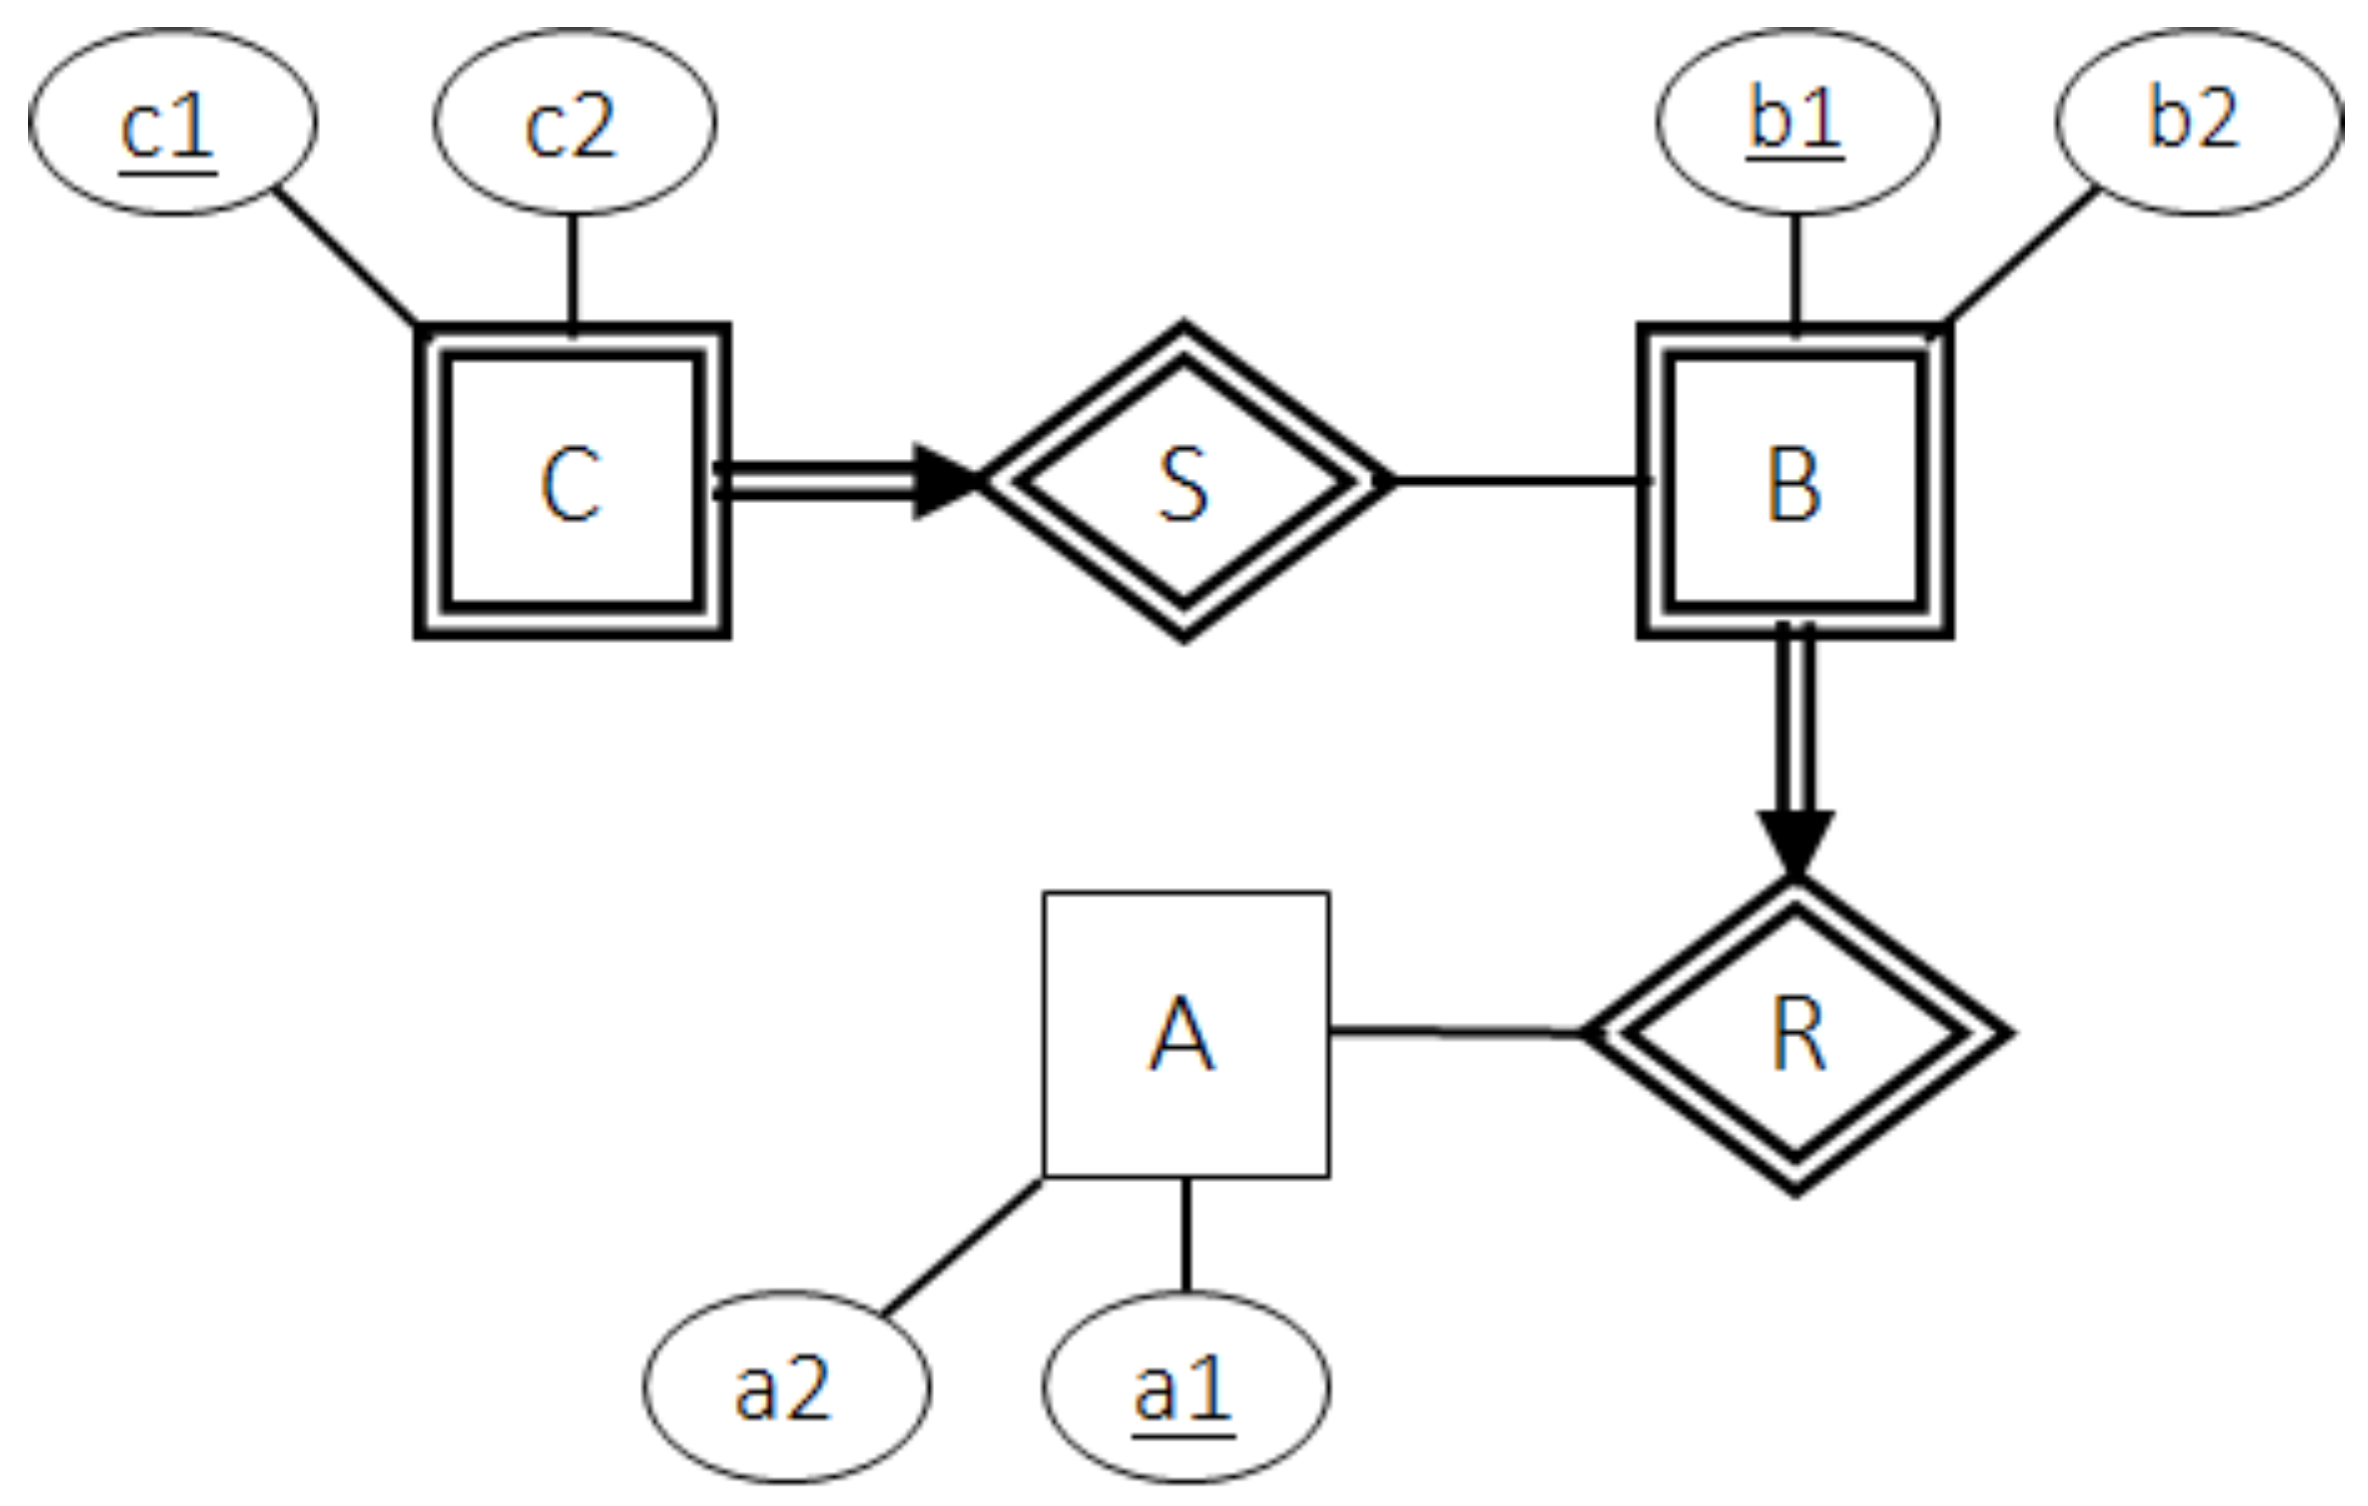
\includegraphics[width=0.95\linewidth]{cs2102-er-model-weak-entity.png} 
    \begin{lstlisting}[style=mySQL, basicstyle=\tiny]
DROP TABLE IF EXISTS A, B, C CASCADE;
CREATE TABLE A (
  a1 INTEGER PRIMARY KEY,
  a2 INTEGER 
);

CREATE TABLE B (
  a1 INTEGER REFERENCES A ON DELETE CASCADE,
  b1 INTEGER,
  b2 INTEGER,
  PRIMARY KEY (a1, b1) 
);

CREATE TABLE C ( 
  a1 INTEGER, 
  b1 INTEGER,
  c1 INTEGER,
  c2 INTEGER,
  PRIMARY KEY (a1, b1, c1),
  FOREIGN KEY (a1, b1) REFERENCES B ON DELETE CASCADE
);
    \end{lstlisting}
  \end{minipage}




\end{multicols}
\end{document}
